 \documentclass[a4paper,14pt]{report}
\usepackage[utf8x]{inputenc} % Включаем поддержку UTF8
\usepackage{extsizes} % Включаем поддержку 14 размера
\usepackage[T2A]{fontenc} % Поддержка русских букв
\usepackage{ucs}
\usepackage[russian, english]{babel}  % Включаем пакет для поддержки русского языка
\usepackage[left=2cm,right=1.5cm,top=1cm,bottom=2cm]{geometry} % Размер отступов
\usepackage{sectsty}
\usepackage[pdftex]{graphicx}
\usepackage{listings}
\usepackage{xcolor}
\usepackage{amsmath}
\usepackage{amsfonts}
\usepackage{enumitem}
\usepackage{cite}
\usepackage{multirow} % улучшенное форматирование таблиц; источник - https://habr.com/post/144648/
\usepackage{indentfirst} % Красная строка
\usepackage[nottoc]{tocbibind}
% \usepackage{flafter}% помещает флоат(изображение) ПОСЛЕ первой ссылки на него; источник - http://mydebianblog.blogspot.ru/2013/03/amorua-advanced-floats.html
% Отображение списка литературы в содержании как section, а не chapter
\makeatletter
\renewenvironment{thebibliography}[1]
     {\section*{\bibname}% <-- this line was changed from \chapter* to \section*
      \@mkboth{\MakeUppercase\bibname}{\MakeUppercase\bibname}%
      \list{\@biblabel{\@arabic\c@enumiv}}%
           {\settowidth\labelwidth{\@biblabel{#1}}%
            \leftmargin\labelwidth
            \advance\leftmargin\labelsep
            \@openbib@code
            \usecounter{enumiv}%
            \let\p@enumiv\@empty
            \renewcommand\theenumiv{\@arabic\c@enumiv}}%
      \sloppy
      \clubpenalty4000
      \@clubpenalty \clubpenalty
      \widowpenalty4000%
      \sfcode`\.\@m}
     {\def\@noitemerr
       {\@latex@warning{Empty `thebibliography' environment}}%
      \endlist}
\makeatother

\setlist{nolistsep} % убрать лишние интервалы в списках
\linespread{1.3} % полуторный интервал
% \renewcommand{\rmdefault}{ftm} % Times New Roman
\lstdefinestyle{sharpc}{language=[Sharp]C, frame=lr, rulecolor=\color{blue!80!black}}
\sloppy


\author{Vladimir Lapatin}
\DeclareGraphicsExtensions{.pdf,.png,.jpg}
\graphicspath{{pics/}}



\begin{document}

\renewcommand{\figurename}{Рисунок} % Замена Figure на Рисунок в подписи изображений

%Титульная страница
\begin{titlepage}	% начало титульной страницы

\begin{center}	
%\\[0.5cm]
\LargeМосковский государственный технический университет имени Н.Э. Баумана\\
\large {(МГТУ им. Н.Э. Баумана)}\\[0.4cm] 
\rule[+3mm]{7.5cm}{0.80mm}
\begin{flushleft}
\begin{tabbing}
ММММММММММ \= \kill
\large{ФАКУЛЬТЕТ} \> \large{\textit{ИНФОРМАТИКА И СИСТЕМЫ УПРАВЛЕНИЯ}} \\	\large{КАФЕДРА} \> \large{\textit{ТЕОРЕТИЧЕСКАЯ ИНФОРМАТИКА}} \\
 \> \large{\textit{И КОМПЬЮТЕРНЫЕ ТЕХНОЛОГИИ}}
\\[1.0cm]
\end{tabbing}
\end{flushleft}
\end{center}


\begin{center}


\Huge{Курсовая работа}\\
\LARGE{<<Приложение хранения библиографических ссылок>>.}
\\[0.5cm]
\LARGE{По курсу <<Базы данных>>.}
\\[2.0cm]




 \rule[+0mm]{6.2cm}{0.0mm}Выполнил:  \rule[+0mm]{1.3cm}{0.0mm} Лапатин В.В.\\
 \rule[+0mm]{6.2cm}{0.0mm}Проверил:  \rule[+0mm]{1.1cm}{0.0mm} Дубанов А.В.\\ [3.5cm]



\large{Москва 2018}
\end{center}
\thispagestyle{empty} % не нумеровать страницу
\end{titlepage} % конец титульной страницы
\clearpage
% -----------------

% Содержание
\renewcommand{\contentsname}{Содержание}
\tableofcontents
\clearpage
% -----------------

% Введение
\section*{Введение}
\addcontentsline{toc}{section}{Введение}

В современном мире каждому приложению необходимо хранить и обрабатывать
различную информацию, что делает чрезвычайно важным понимание разработчиком принципов работы с информацией. Для этого
необходимо знать о различных средствах хранения информации и иметь представление о механизмах их работы. Также важным является
умение разрабатывать серверные приложения, которые осуществляют взаимодействия с базами данных.

Таким образом, цель данной курсовой работы заключается в изучении различных средств хранения информации, создании базы
данных и разработке приложений, предоставляющих инструменты для работы с сохраненными данными.

Постановку задачи можно сформулировать следующим образом:
необходимо разработать приложение, которое выполняет генерацию списков литературы
для учебных курсов в формате BibTeX. Для этого приложение должно иметь следующие функции:

\begin{enumerate}
    \item Поиск информации о книгах.
    \item Хранение и модификация информации о книгах.
    \item Создание и модификация данных об учебных курсах.
    \item Генерация списка литературы.
\end{enumerate}
\clearpage
% -----------------

% Глава 1
\section*{Разработка интерфейса}
\addcontentsline{toc}{section}{Разработка интерфейса}

Для любой программы интерфейс является одной из наиболее важных составляющих.
Ведь именно он определяет, как приложение будет взаимодействовать с другими
программами и своими пользователями. Таким образом, можно ввести следующую
классификацию интерфейсов:

\setlist{nolistsep}
\begin{enumerate}
    \item программные,
    \item графические,
    \item интерфейсы командной строки.
\end{enumerate}

Несмотря на то, что эти интерфейсы имеют между собой мало общего, к ним 
предъявляется ряд общих требований:

\begin{enumerate}
    \item функциональность -- интерфейс должен отвечать всем требованиям пользователя и соответствовать его задачам,
    \item логичность -- интерфейс должен быть логичным и запоминающимся, чтобы взаимодействие пользователя
        с программой было как можно более простым и удобным,
    \item защищенность -- интерфейс должен быть спроектирован таким образом, чтобы у пользователя не было
        возможности совершить ошибку.
\end{enumerate}

После определения общих требований к любому интерфейсу, стоит рассмотреть перечисленные выше
интерфейсы отдельно.

\subsection*{Программные интерфейсы}
\addcontentsline{toc}{subsection}{Программные интерфейсы}

К программным интерфейсам можно причислить любой интерфейс, который предназначен для
использования разрабатываемой программы внешними приложениями. Обычно, в зависимости от
используемых технологий, это набор классов, функций или методов, которые используются
внешними программами. В случае данного приложения в качестве интерфейса взаимодействия
было решено использовать веб-технологии. Это означает, что приложение будет взаимодействовать
с любыми своими пользователями через протокол HTTP.
Таким образом, программный интерфейс приложения будет представлять из себя набор HTTP-методов.

В протоколе HTTP есть несколько видов методов, из которых приложением будут использоваться следующие:

\begin{enumerate}
    \item GET -- это методы, которые запрашивают данные, они не предназначены для их записи,
    \item POST -- это методы, которые используются и для записи данных, и для их получения.
\end{enumerate}

Говоря об HTTP интерфейсах, стоит отметить, что есть несколько различных подходов к проектированию
подобных интерфейсов. Одним из наиболее общепринятых подходов является так называемый REST.
Это можно перевести как Represental State Transfer\cite{REST}. Данная архитектура предлагает
наложить на приложение ряд следующих ограничений:

\begin{enumerate}
    \item модель клиент-сервер -- означает, что вся логика должна выполняться на удаленном сервере,
    а клиентское приложение должно исключительно предоставлять и получать данные,
    \item отсутствие состояния -- сервер получает из запроса всю необходимую информацию и не хранит
    никакую информацию о сессии клиентов,
    \item кэширование -- сервер сохраняет наиболее частые ответы, что позволяет не выполнять
    лишние запросы к базе данных и соответствующие вычисления, а сразу вернуть результат,
    \item единообразие интерфейса,
    \item слои -- сокрытие основного сервера за промежуточными. Например, без каких-либо
    изменений для пользователя можно внедрить между ним и сервером промежуточный сервер, который
    предназначен для хранения и отдачи хэшированных данных. В случае отсутствия этих данных
    хэширующий сервер перенаправляет запрос исходному серверу.
\end{enumerate}

Такой подход позволяет добиться лучшей производительности за счет отсутствия состояний между
вызовами и кэширования, а архитектура становится более расширяемой из-за требований
единообразия и использования слоев.

\subsection*{Графические интерфейсы}
\addcontentsline{toc}{subsection}{Графические интерфейсы}

Графические интерфейсы -- это наиболее востребованные интерфейсы в современном мире, потому
что пользователям намного более удобно пользоваться интерфейсами, у которых среди
средств донесения информации есть не только текст. 

И, пожалуй, самый популярный вид графических приложений -- это веб-сайты.
Они получили такую популярность из-за своей универсальности: пользователь
может открыть приложение на любом устройстве, на котором есть доступ в интернет
и веб-браузер, в то время как любое другое приложение потребует установки
на устройство пользователя. С другой стороны, веб-сайты очень удобны для
разработчиков. Намного более выгодно разработать одно веб-приложение, чем
создавать и поддерживать несколько программ для разных платформ.

Обычно разработку веб-приложения можно разделить на две части:
<<фронтенд>> и <<бэкенд>>.

<<Фронтенд>> -- это та часть приложения, которая исполняется в браузере пользователя.
Для написания веб-сайтов используются язык разметки HTML, язык описания стилей CSS и интерпретируемый
язык программирования JavaScript.

Опишем роль каждого языка в веб-приложении:
\begin{enumerate}
    \item HTML -- это каркас всего приложения, который определяет, какие элементы будут использоваться и
    где они будут располагаться,
    \item CSS определяет, как будут выглядеть элементы приложения. Сюда входят, например, внешний вид кнопок
    или вид шрифта отображаемого текста,
    \item JavaScript -- это интерпретируемый язык программирования, основная область применения которого заключается
    в придании интерактивности веб-страницам. Например, динамическую загрузку данных в таблицу можно реализовать только
    через JavaScript. 
    
\end{enumerate}

<<Бэкендом>> обычно называют ту часть приложения, которая стоит за <<фронтендом>>. В основном это
та программа, которая предоставляет данные, выполняет их хранение и агрегацию. Другими словами,
<<бэкенд>> реализует всю <<бизнес-логику>>, в то время как <<фронтент>> нужен для предоставления
пользователям доступа к приложению. Более подробно об этом будет рассказано далее.

\subsection*{Интерфейсы командной строки}
\addcontentsline{toc}{subsection}{Интерфейсы командной строки}

Интерфейсы командной строки, в отличии от графических и программных интерфейсов, представляют
наименее популярную группу приложений. Но, несмотря на это, они являются
незаменимыми. Главное преимущество приложений командной строки заключается в том, что
ими могут пользоваться в равной степени эффективно человек, и программа. Таким образом,
интерфейсы командной строки являются сочетанием программных и графических интерфейсов:
с одной стороны ими с определенной степенью удобства может пользоваться человек, а с другой
стороны без каких-либо трудностей они могут использоваться для взаимодействия между
приложениями. Также стоит отметить, что приложениям командной строки не нужен какой-либо
графический интерфейс, только окно терминала.

Для того, чтобы заниматься непосредственным проектированием интерфейсов, необходимо
понять задачу, которые они будут решать.

\subsection*{Постановка задачи}
\addcontentsline{toc}{subsection}{Постановка задачи}

Необходимо разработать приложение, которое выполняет генерацию списков литературы
для учебных курсов в формате BibTeX. Для этого приложение должно иметь следующие функции:

\begin{enumerate}
    \item Поиск информации о книгах;
    \item Хранение и модификация информации о книгах;
    \item Создание и модификация данных об учебных курсах;
    \item Генерация списка литературы.
\end{enumerate}

\subsection*{Разработка программного интерфейса}
\addcontentsline{toc}{subsection}{Разработка программного интерфейса}

При рассмотрении программных интерфейсов была описана архитертура REST. Согласно
этой архитектуре каждый метод должен принимать в себя всю необходимую информацию
для выполнения запроса, а все методы должны быть унифицированы. Таким образом, для каждого
вида данных был реализован следующий набор методов:

\begin{itemize}
    \item add\%Имя таблицы\% -- POST запрос, содержащий данные для добавления в теле,
    \item get\%Имя таблицы\% -- GET запрос, получающий данные от приложения,
    \item prototype\%Имя таблицы\% -- GET запрос, получающий прототип JSON-файла для искомой таблицы.
\end{itemize}

Также были реализованы две дополнительных команды: report и migrate.

Первая получает данные, необходимые для однозначной идентификации требуемого списка литературы
и генерирует для этого списка литературы файл в формате BibTeX. 

Команда migrate выполняет копирование списка литературы с одного года на другой. Это необходимо для того,
чтобы облегчить работу пользователя, ведь обычно учебные программы слабо меняются от года к году.

\subsection*{Разработка интерфейса командной строки}
\addcontentsline{toc}{subsection}{Разработка интерфейса командной строки}

Как уже было сказано выше, для интерфейсов командной строки крайне важна автоматизируемость.
Это делает невозможным использование так называемого интерактивного ввода. Другими словами,
любое действие пользователя должно совершаться за один вызов приложения. В результате
было решено использовать следующий подход к проектированию интерфейса: для каждого вида данных,
с которыми будет работать приложение, будет реализована собственная команда. И для каждой такой
команды будет реализован набор подкоманд, выполняющих необходимые действия. В общем случае
команду приложения командной строки можно описать в следующем виде:

\begin{itemize}
    \item \%Имя таблицы\% prototype -- данный метод добавляет новый файл в файловую систему,
        который содержит в себе прототип для нужного вида данных. После чего пользователь
        должен заполнить этот прототип информацией, которую хочет добавить,
    \item \%Имя таблицы\% add -- сохраняет данные в приложение,
    \item \%Имя таблицы\% get -- позволяет получить данные из приложения, можно конфигурировать
        флагами.
\end{itemize}

Также отличительной чертой хорошего приложения командной строки является грамотно оформленная справка.
Рисунок ~\ref{ris:help_example} показывает результат выполнения команды help. 

\begin{figure}[h!]
    \center{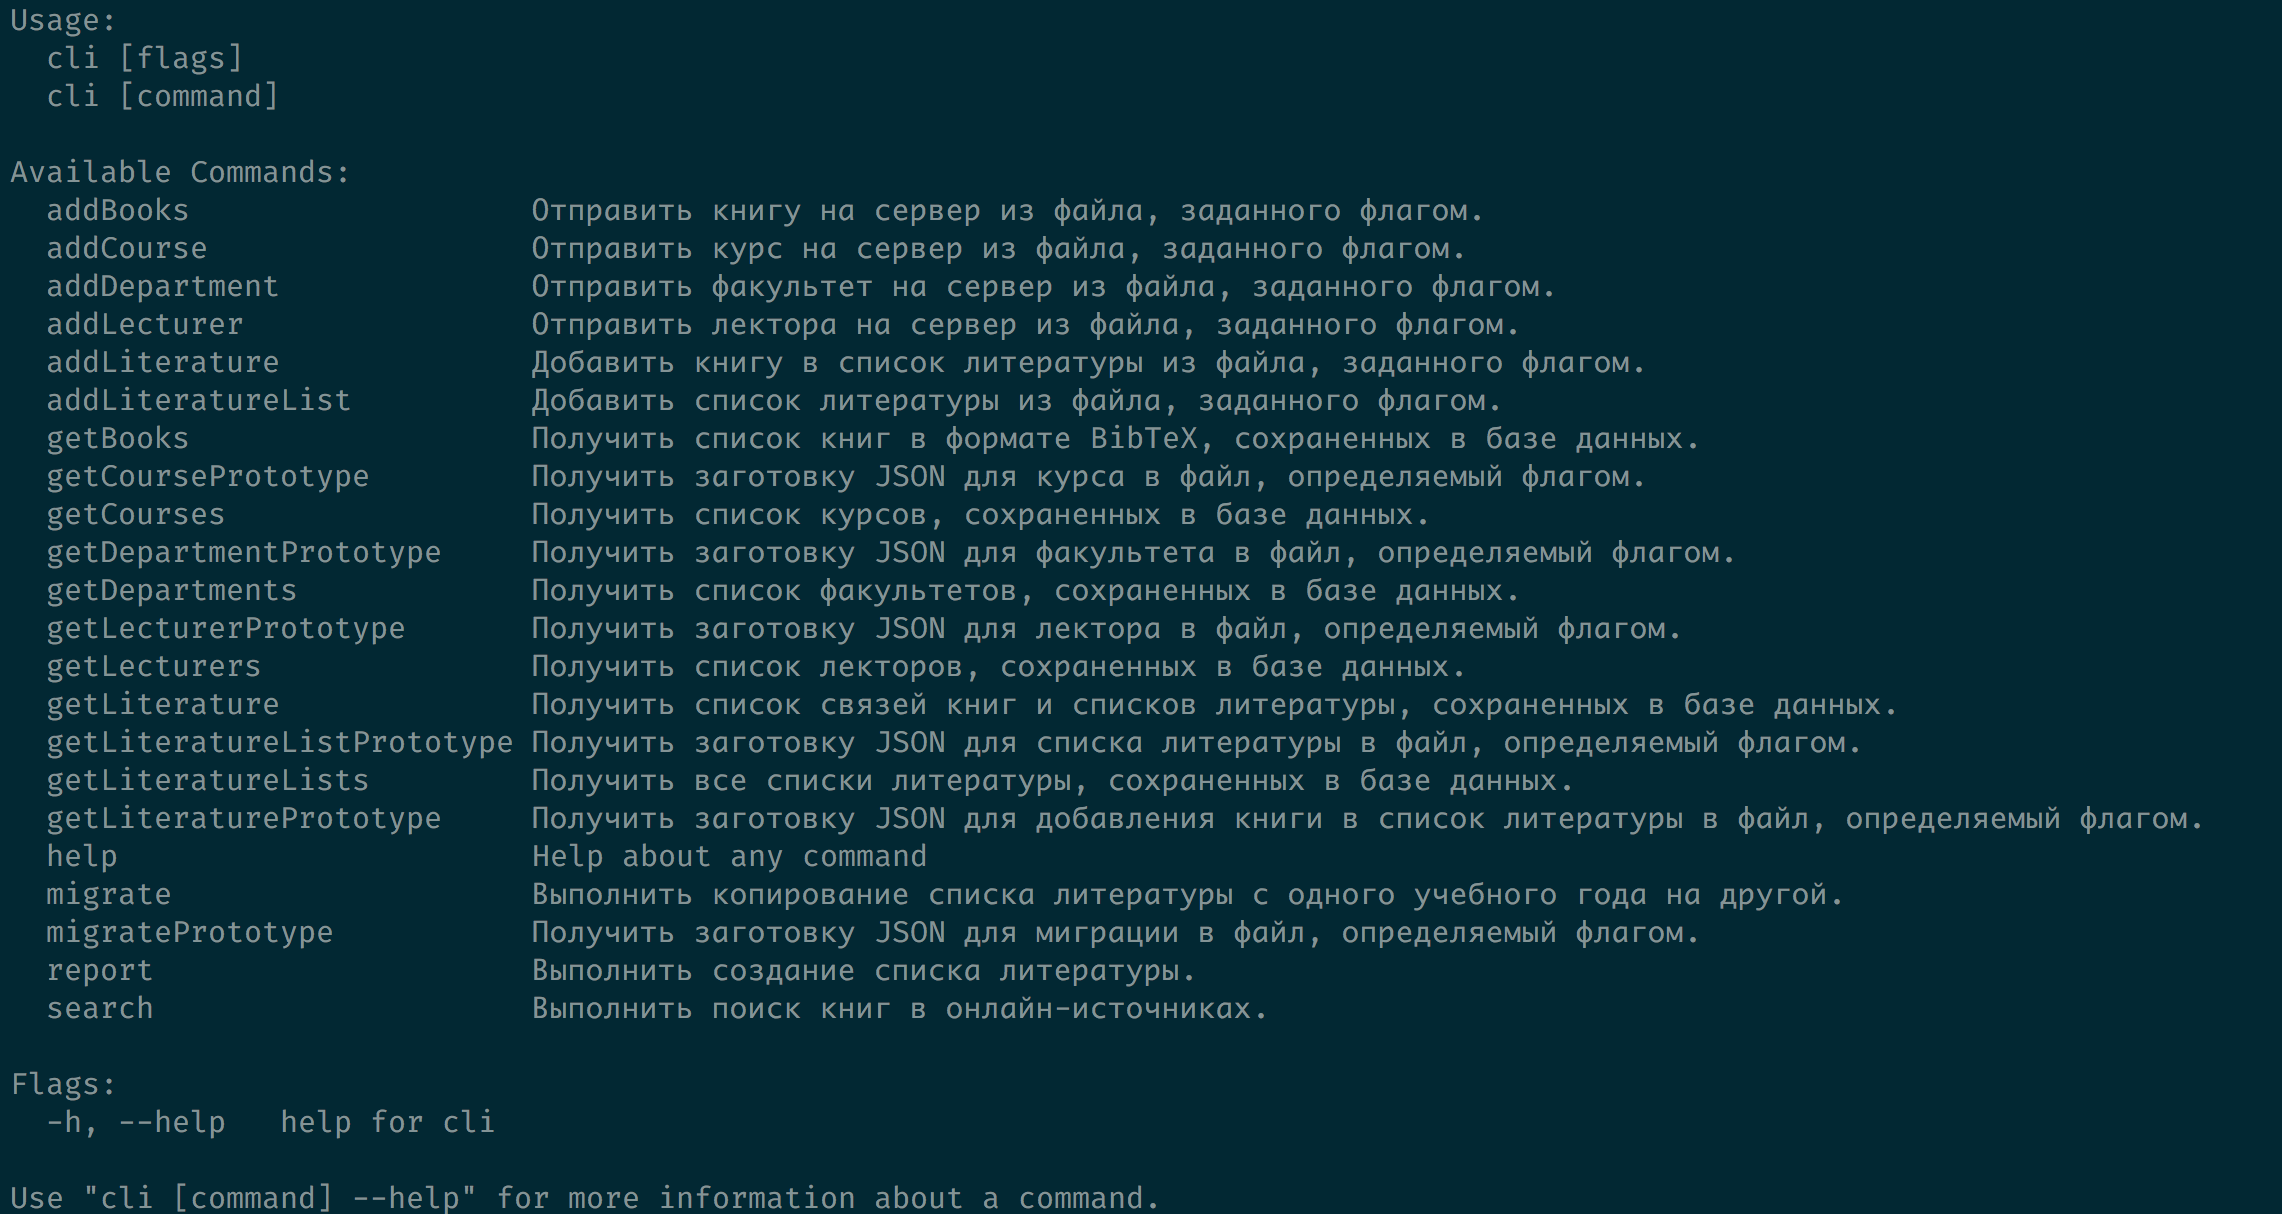
\includegraphics[width=1\linewidth]{help}}
    \caption{Пример работы команды help.}
    \label{ris:help_example}
\end{figure}

Также для каждой отдельной команды реализован
отдельный флаг --help, который показывает справку для конкретной команды, что можно видеть на рисунке 
~\ref{ris:help_book_example}. 

\begin{figure}[h!]
\center{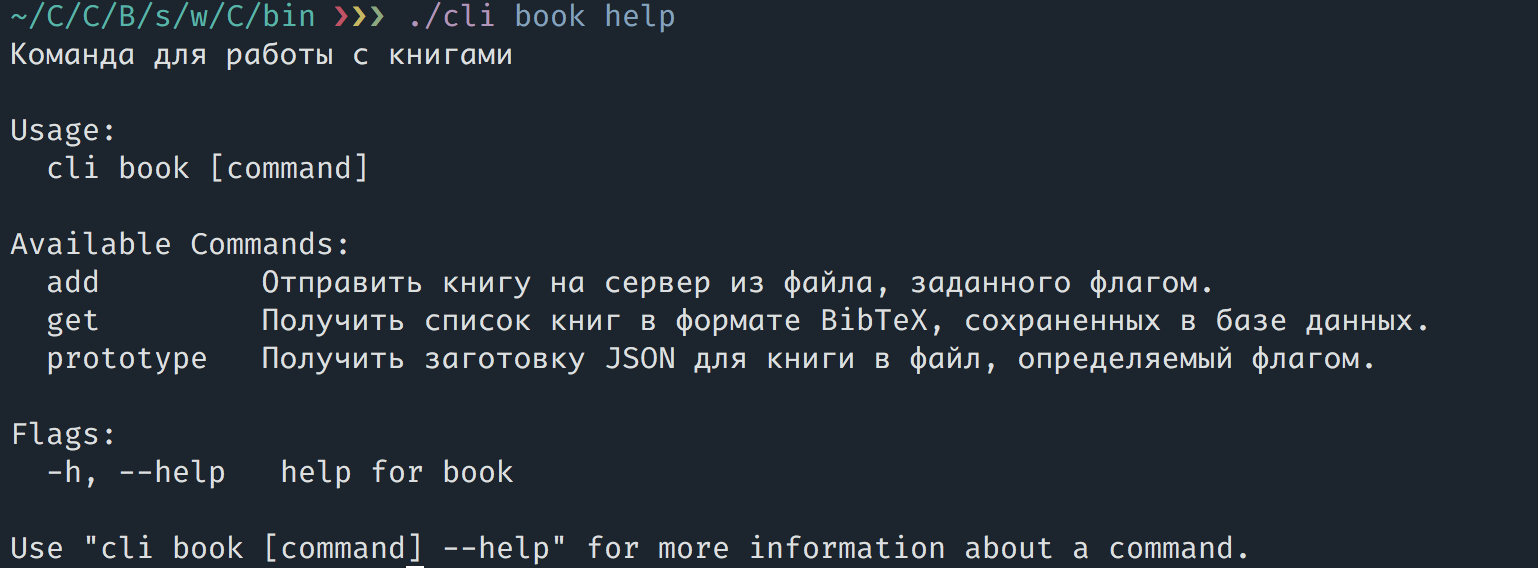
\includegraphics[width=1\linewidth]{help_book}}
\caption{Пример работы флага help для команды book}
\label{ris:help_book_example}
\end{figure}


//Описать дополнительные команды вроде migrate и generate; сделать скриншоты работы программы

\subsection*{Разработка графического интерфейса}
\addcontentsline{toc}{subsection}{Разработка графического интерфейса}

Как уже было сказано выше, графический интерфейс реализован в виде веб-сайта, написанного на языке TypeScript с 
использованием фреймворка Bootstrap.
Выбор фреймворка обусловлен тем, что он предоставляет продвинутый набор стилей и HTML-элементов, что позволяет 
легко и быстро настроить внешний вид веб-приложения.
В связи с тем, что единственный современный и поддерживаемый язык для написания веб-сайтов - это JavaScript, то 
из альтернатив ему можно использовать только языки, компилируемые в JavaScript. В частности, к таким языкам можно 
отнести язык TypeScript компании Microsoft и язык Kotlin, разрабатываемый компанией JetBrains, который имеет 
отдельный плагин для компиляции JS-код. К сожалению, Kotlin является очень молодым языком, который находится в 
активной разработке, так что было решено использовать TypeScript. Преимуществом данного языка является то, что 
он является надмножеством JavaScript. Это означает, что любой JavaScript код является абсолютно корректным. Также 
важно отметить, что TypeScript поддерживает важные аспекты объектно-ориентированого программирования: классы, 
инкапсуляцию(уточнить насчет остального). Но главным преимуществом этого языка является его строгая типизированность. 
Это облегчает разработку и позволяет писать более читаемый код по сравнению с JavaScript.

На рисунках ~\ref{ris:web_example_1} и ~\ref{ris:web_example_2} видно, приложение состоит из четырех логический частей. 

\begin{figure}[h!]
    \center{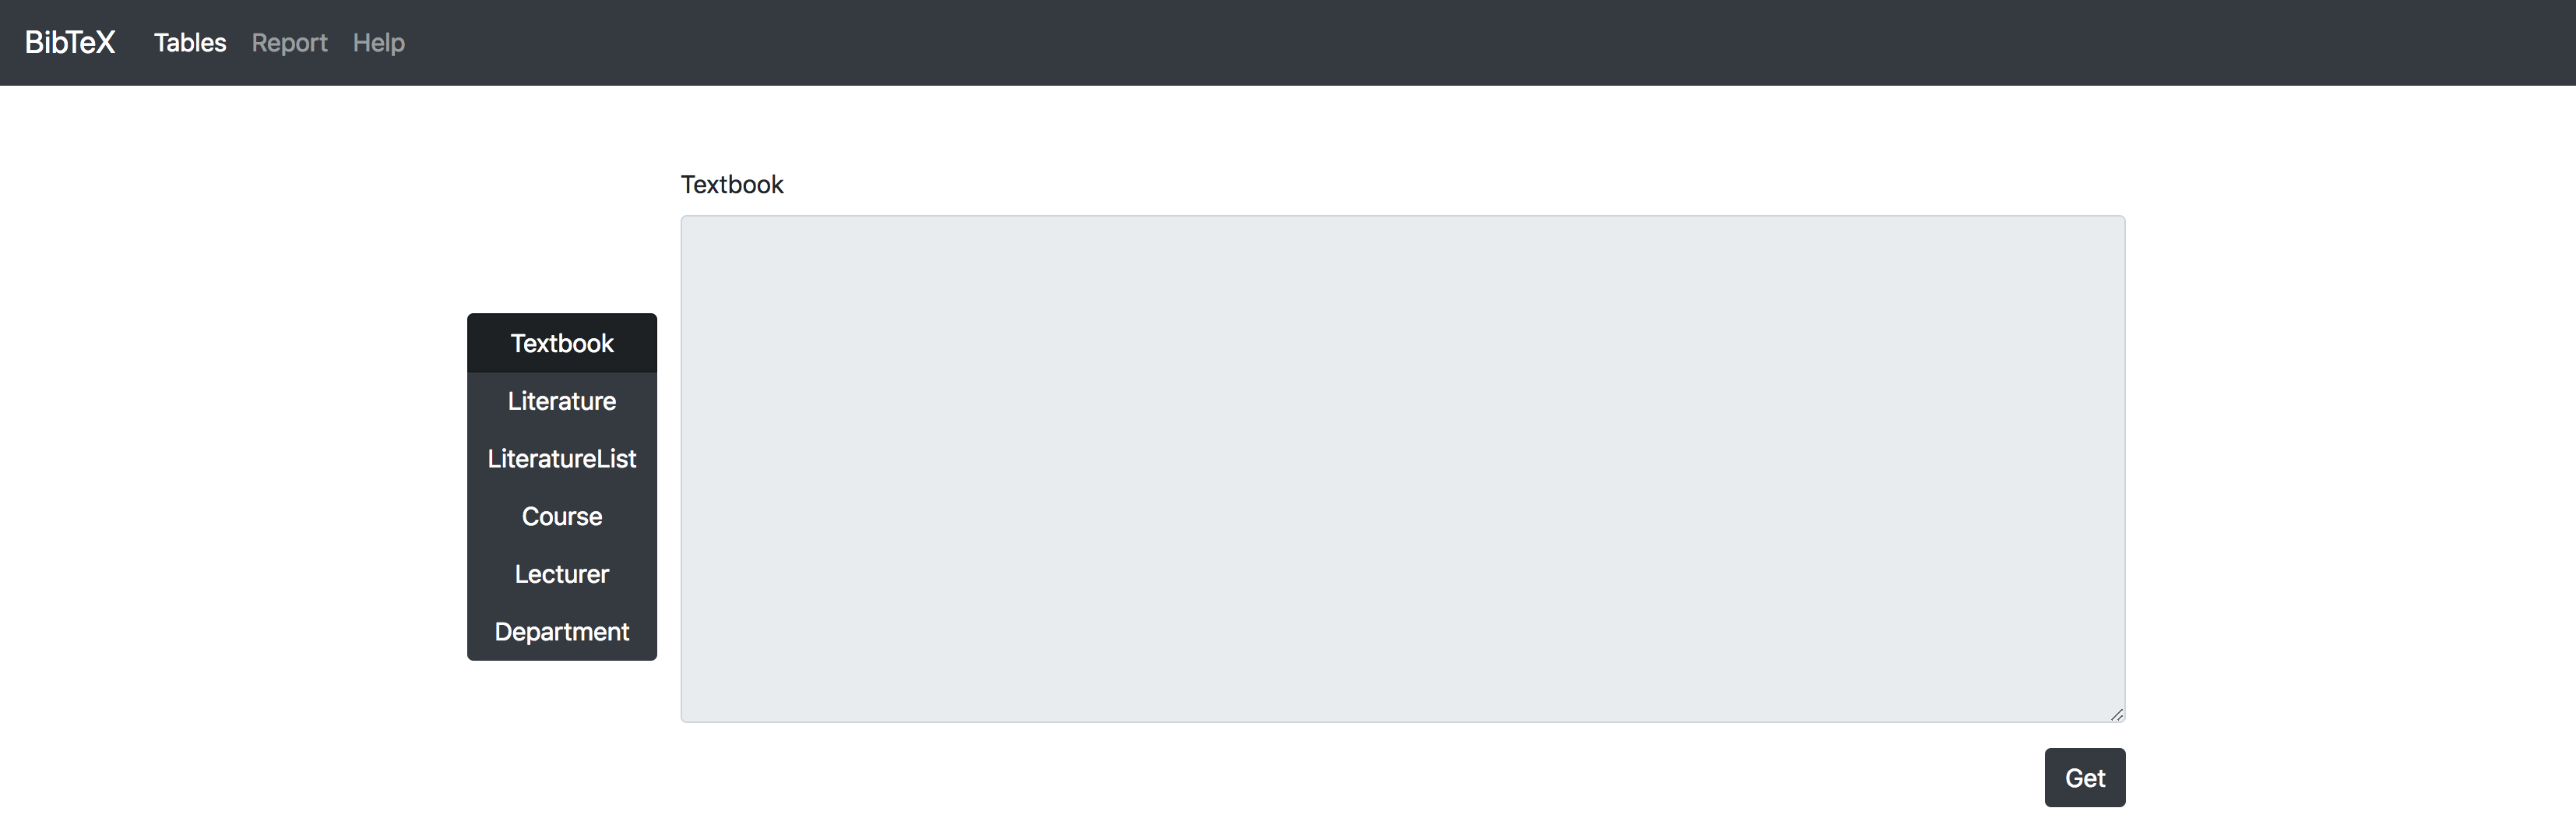
\includegraphics[width=0.8\linewidth]{web_example_1}}
    \caption{Верхняя часть веб-сайта}
    \label{ris:web_example_1}
\end{figure}

\begin{figure}[h!]
    \center{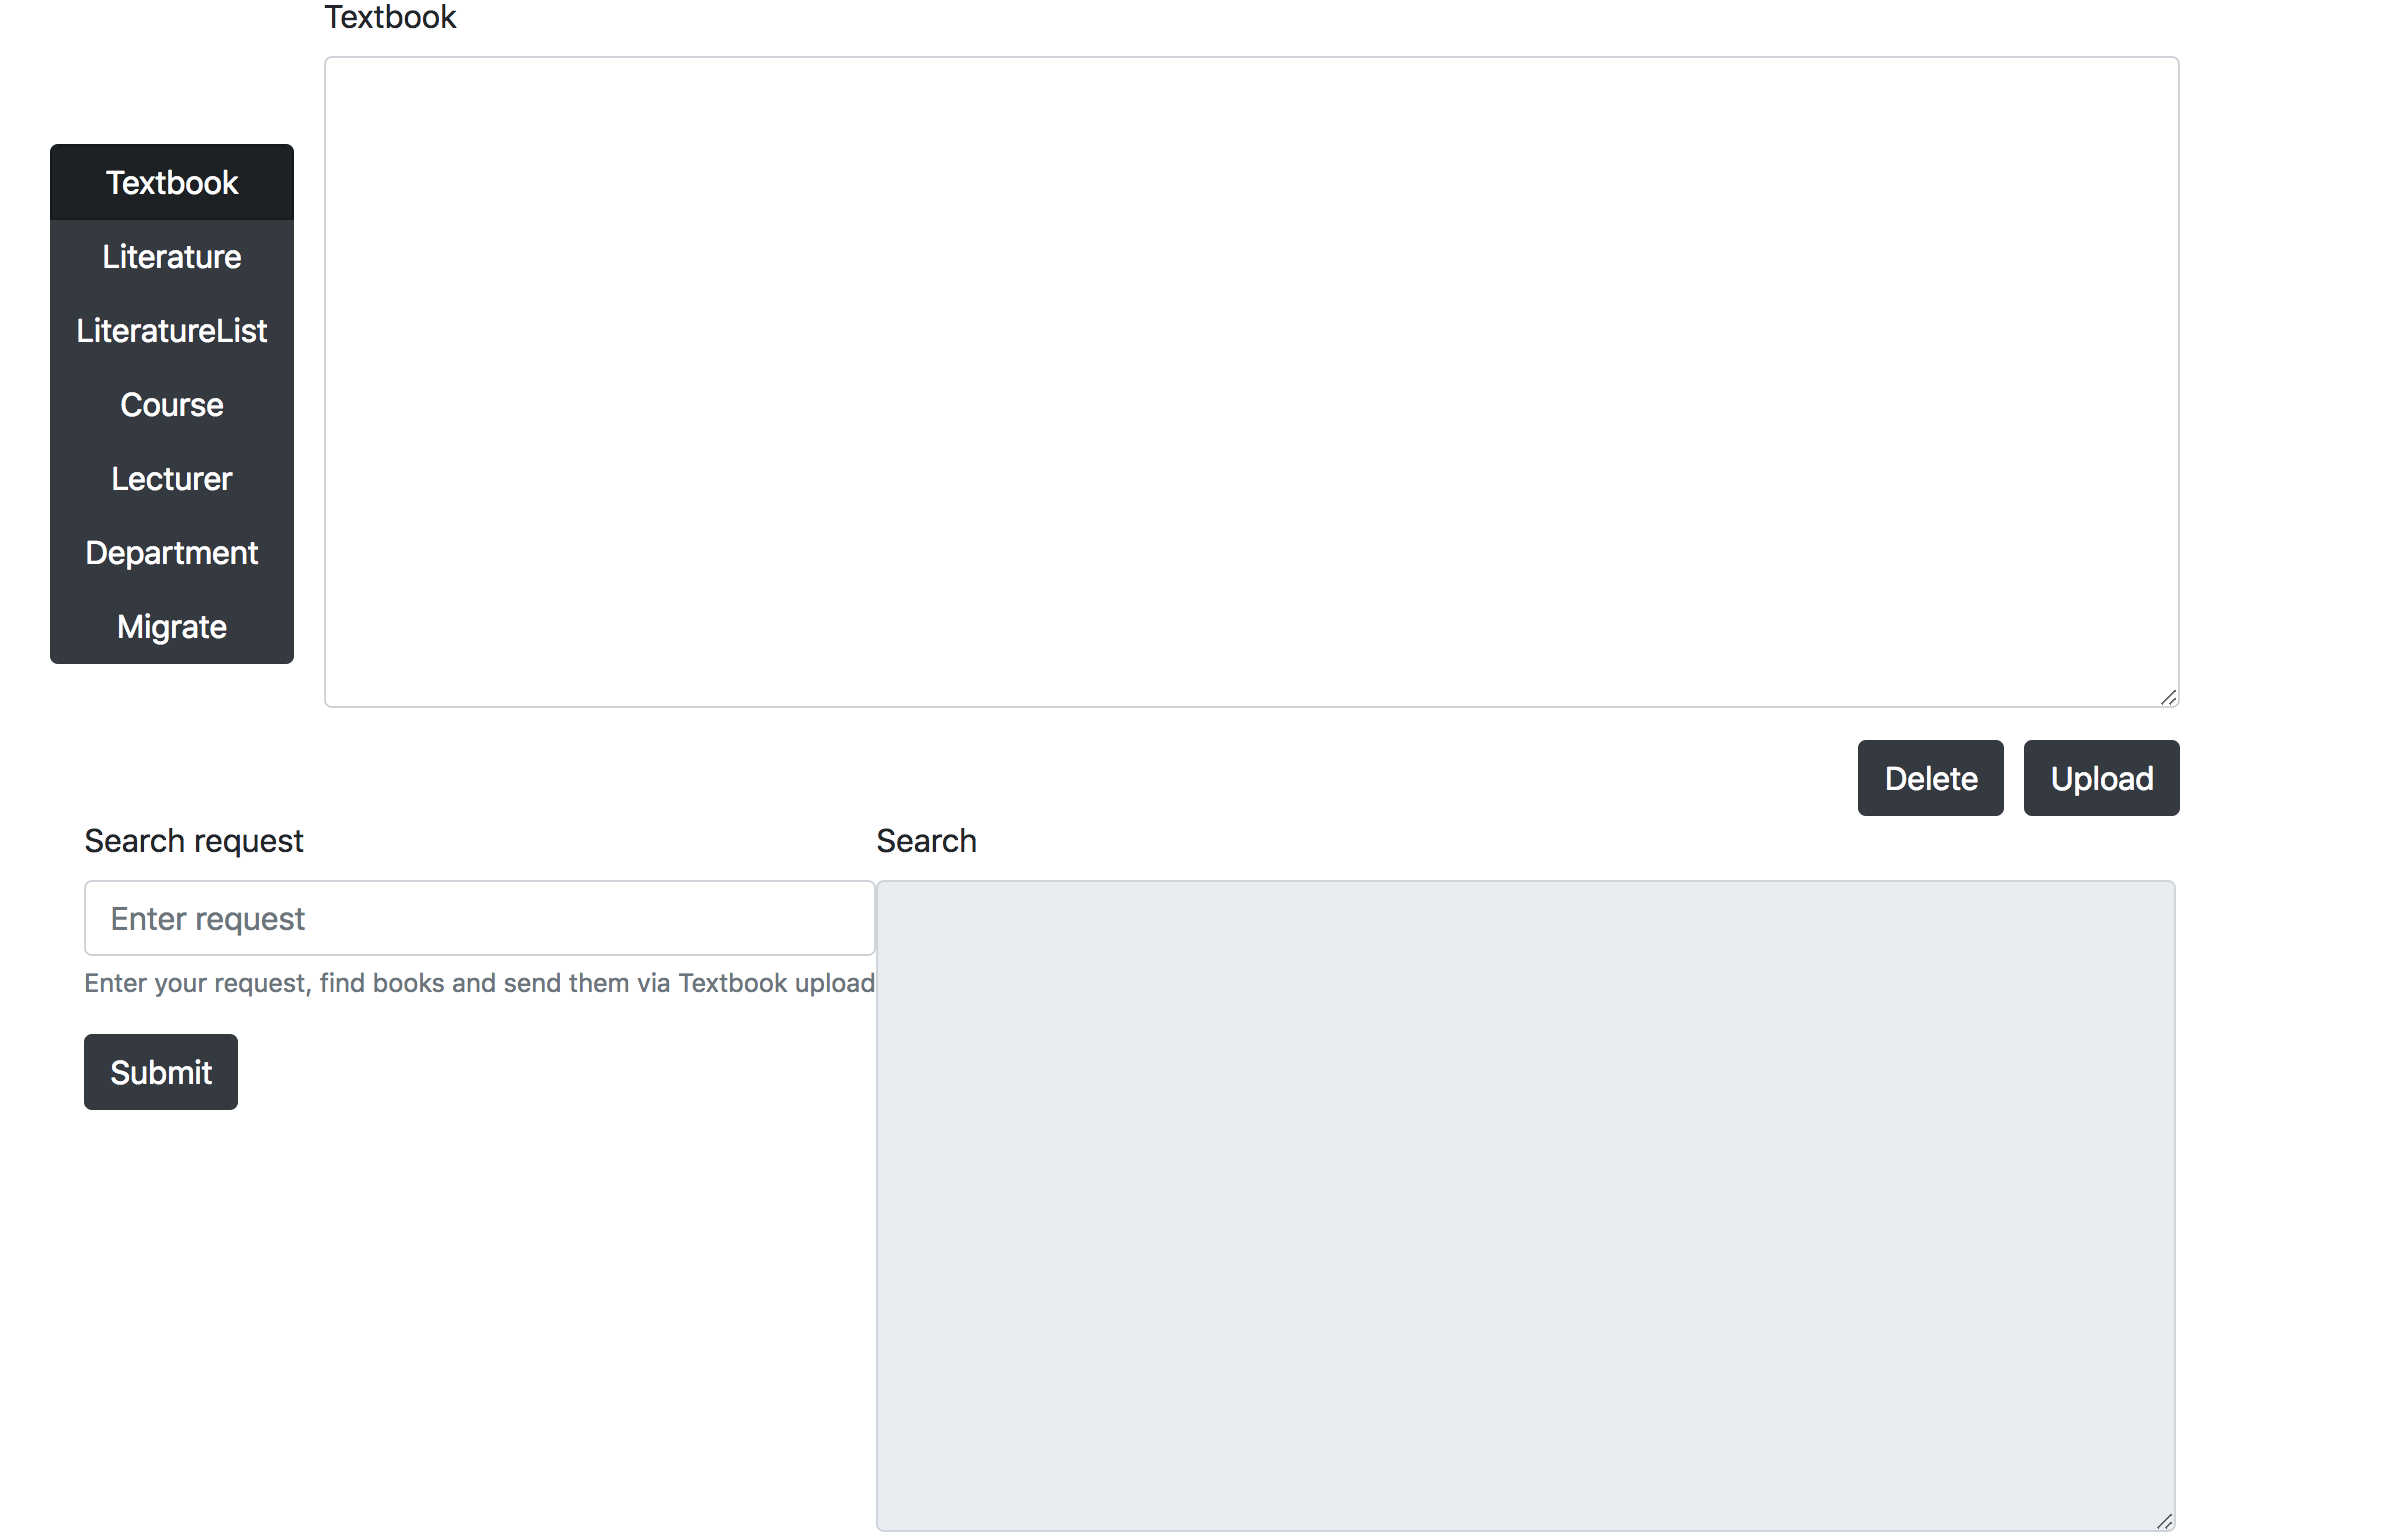
\includegraphics[width=0.8\linewidth]{web_example_2}}
    \caption{Нижняя часть веб-сайта}
    \label{ris:web_example_2}
\end{figure}

Первая - шапка сайта. Она содержит название 
приложения и ссылки на три страницы приложения: основную рабочую область, страницу генерации отчетов и страницу со 
справкой.

Вторая логическая часть - это большая недоступная для ввода область TextArea вместе с набором кнопок, 
отвечающих за переключение используемой таблицы. Эта часть нужна для получения данных, которые 
уже содержатся в базе данных для более удобного добавления новых записей в приложение.

Третья часть -- доступная для ввода область TextArea, в которую автоматически загружаются
JSON прототипы для текущего вида входных данных.

Заключительная область необходима для поиска необходимых книг в сервисе Google Books.

\clearpage
% -----------------

% Глава 2
\section*{Проектирование базы данных}
\addcontentsline{toc}{section}{Проектирование базы данных}

База данных является неотъемлемой частью любого приложения, которое выполняет
хранение и обеспечивает работу с информацией. Так что выбор правильной технологии
хранения данных является чрезвычайно важной задачей. 

На текущий момент существует две различные ветви развития систем управления
базами данных(СУБД): релационная и нереляционная.

Отличительной чертой реляционных баз данных является понятие отношения или таблицы.
Каждая сущность, хранимая в базе данных, должна представлять собой строку таблицы со 
строго заданным типизированным набором столбцов. Также реляционные СУБД гарантируют
выполнение так называемых свойств ACID к транзакционной системе, где под транзакцией
понимается последовательность команд, представляющая логическую единицу работы с данными.
Опишем свойства ACID: 

\begin{enumerate}
    \item Атомарность -- транзация либо будет выполнена целиком, либо
        не выполнена совсем;
    \item Согласованность -- после выполнения транзакции в базе данных
        находятся корректные значения;
    \item Изолированность -- на транзакцию не могут оказать влияния другие транзакции,
        выполняемые параллельно;
    \item Устойчивость -- если транзакция была завершена, то даже при сбое системы
        изменения будут зафиксированы.
\end{enumerate}

Данные свойства накладывают довольно серьезные ограничения на производительность, что
послужило поводом для появления нереляционных СУБД. Перед ними стояло требование
обеспечить хранение данных для высоконагруженных приложений. В противовес
свойствам ACID, нереляционные базы данных гарантируют выполнение свойств BASE
(Источник: What NoSQL is and what it is not.):

\begin{enumerate}
    \item Доступность -- каждый запрос будет выполнен;
    \item Гибкость -- состояние системы может меняться со временем даже без ввода новых данных;
    \item Согласованность в конечном счете -- данные могут быть несогласованны в некоторые
        моменты времени, но в итоге приходят в согласованное состояние.
\end{enumerate}

//Проверить точность формулировок в первоисточнике

Стоит отметить, что существует множество видов нереляционных баз данных, перечислим
основные:

\begin{enumerate}
    \item документоориентированные;
    \item графовые;
    \item ключ-значение;
\end{enumerate}

Графовые базы данных не дадут особого выигрыша из-за относительной простоты хранимых данных.

В произведенном далее сравнении все замечания, относящиеся к документоориентированным базам данных
в равной степени относятся и к базам данных вида ключ-значения, так что ниже речь будет идти
только о реляционных и документоориентированных СУБД.

Для того, чтобы избежать голословности, сравнение будет проводиться на примере реляционной СУБД PostreSQL и 
нереляционной MongoDB.

В основе документоориентированной базы данных лежит понятие документа. В общем случае в качестве формата
может быть множество различных стандартов: JSON, XML, YAML и так далее. В случае MongoDB для хранения
используется BSON -- надмножество JSON. В данной СУБД документы группируются в так называемые
коллекции. В отличии от реляционной модели, коллекция не имеет какой-либо строгой структуры. То есть
в ней могут храниться абсолютно разные документы.

Данных подход имеет ряд своих преимуществ и недостатков. Перечислим положительные стороны:

\begin{enumerate}
    \item гибкость -- так как коллекция не ограничена структурой хранимых данных, информация
        в ней может несколько отличаться от записи к записи. Это может полезно, если
        данные имеют в целом общий смысл, но в некоторых документах могут присутствовать
        какие-то особые поля;
    \item производительность -- так как не происходит никаких проверок, запись и чтение
        работают существенно быстрее, чем в реляционном подходе;
\end{enumerate}

Недостатки и ограничения:

\begin{enumerate}
    \item Подобная организация плохо подходит для создание ссылок между объектами по, например,
        первичному ключу. Это связано с описанным выше отсутствием проверок. Канонический
        способ хранения данных -- это использование вложенных документов. Но этот способ
        применим не везде из-за ограничение на размер документа в 16 МБ.
    \item Как было описано в пункте выше, довольно сложно производить нормализацию
        данных, потому что все проверки необходимо производить не на уровне СУБД, а
        на уровне приложения.
\end{enumerate}

После анализа плюсов и минусов NoSQL подхода стоит определить, какие данные будут храниться
и какие требования должны соблюдаться.

В первую очередь стоит отметить, что все данные имеют абсолютно строгую структуру. Если говорить
о хранимых книгах, то для них есть набор полей, определяемый стандартном BibTeX, который обязан
быть у каждой записи. Остальные данные, такие как списки литературы и учебные курсы, также не имеют
никакой вариативности. Таким образом, гибкость NoSQL подхода только добавит сложностей в связи
с необходимостю ручной реализации множества проверок.

А во вторую очередь нужно сказать, что конечная цель приложения -- генерировать списки литературы
для учебных курсов. И весьма логичным требованием будет то, что в любой момент времени приложение
должно генерировать корректные отчеты. Таким образом, для данной задачи больше подходят требования
ACID, чем BASE.

Как видно из рассуждений выше, несмотря на все свои преимущества, для поставленной задачи больше
подходит реляционная модель.

Следующий этап проектирования -- это формализация таблиц базы данных. Перечислим таблицы и их
их цели:

\begin{itemize}
    \item Textbook -- таблица с книгами в формате BibTeX. Обладает несколькими UNIQUE столбцами:
        \begin{itemize}
            \item ident -- идентификатор книги, должен быть уникальным, так как именно
                он используется для идентификации библиографической ссылки в стандарте LaTeX;
            \item isbn -- уникальный для каждой книги ключ, позволяет исключить дублирование;
        \end{itemize}
    \item LiteratureList -- таблица, хранящая списки литературы. Имеет UNIQUE ограничение на
        пару из ID курса, которому присвоем список и года этого курса. Это необходимо для
        идентификации списка литературы;
    \item Literature -- так называемая таблица пересечения, необходимая для создания связи
        многие-ко-многим между таблицами LiteratureList и Textbook;
    \item Course -- задает учебный курс. Стоит отметить, что один учебный курс может иметь
        несколько списков литературы за разные года. Имеет ссылки на кафедру, к которой 
        привязан и лектора, читающего курс. Обладает UNIQUE ограничением на тройку из
        названия, кафедры и семестра, в котором читается курс;
    \item Department -- задает кафедру, имеет UNIQUE поле title, характеризующее
        название кафедры;
    \item Lecturer -- хранит всех лекторов. Однозначно идентифицируется именем и датой рождения.
\end{itemize}

Все таблицы обладают суррогатными первичными ключами.

Стоит также отметить два важных решения, которые были приняты для всей базы данных.
Во-первых, каждая запись имеет поле timestamp -- временную метку добавления или изменения записи.
Это позволит иметь историю изменений. Также нужно уточнить, что данное поле имеет тип integer,
что является более общим решением, чем хранение метки во внутреннем формате СУБД.
Во-вторых, в базе данных будет отсутствовать возможность удаления записи. Для этого каждая
запись имеет флаг isDeleted. При удалении пользователем записи она будет помечаться, как удаленная.
У данного решения есть ряд преимуществ. Это позволяет обезопасить базу данных от ошибок пользователя
и от потенциального взлома системы. И в том, и в другом случае никому не удастся нанести
непоправимый ущерб данным. Причем блокировка будет осуществляться за счет того, что у учетной записи,
через которую пользователь будет взаимодействовать с базой данных, не будет прав на удаление из базы данных.
При этом все равно будет администратор, у которого данная возможность есть.
\clearpage
% -----------------

% Глава 3
\section*{Разработка серверного приложения}
\addcontentsline{toc}{section}{Разработка серверного приложения}

Разработанное серверное приложение можно разделить на несколько модулей или пакетов языка Go, что и было сделано
в исходном коде программы. В первую очередь стоит отметить пакет \texttt{fetcher}, который отвечает за
поиск книг в сервисе Google Books. Все, что он делает: формирует запрос с помощью API-ключа и данных,
введенных пользователем, после чего отправляет его и получает ответ, а дальше возвращает его в необходимом
формате. Именно по этой причине для старта приложения необходимо вводить API-ключ.

Далее следует, пожалуй, самая крупная часть данного приложения: работа с базой данных. Как уже было упомянуто
выше, работа с базой данных ведется с использованием связки из модуля стандартной библиотеки \texttt{database/sql} и
драйвера \texttt{pq}. Пакет \texttt{database/sql} является исключительно интерфейсом, в то время как именно
драйвер реализует всю необходимую логику. Для их взаимодействия нужно добавить в файл оба этих пакета, используя команду
\texttt{import}.

Для начала будет правильным рассмотреть принципы работы с \texttt{database/sql}.
Подключение к СУБД происходит с помощью метода \texttt{sql.Open}.
Данный метод имеет два параметра:

\begin{itemize}
    \item имя драйвера -- в данном случае это будет postgres
    \item конфигурационная строка -- набор пар ключ-значение, определяющее все параметры подключения. Например,
    подключение к базе данных <<bibtex>> пользователя <<username>> к СУБД, находящейся на порту 8888, будет выглядеть
    следующим образом: "user=username port=8888 dbname=bibtex"
\end{itemize}

Метод \texttt{sql.Open} вернет структуру \texttt{sql.DB}, через которую будут происходить
все дальнейшие взаимодействия с СУБД, в частности, внесение и получение данных.

Следующим шагом стоит выполнить метод \texttt{DB.Ping}, который создает или восстанавливает подключение.
Это позволяет удостовериться, что все работает корректно. После этого СУБД готова к использованию в приложении.

В первую очередь при разработке были реализованы методы \texttt{insert} и \texttt{select} для всех таблиц.
Стоит отметить, что приложение рассчитано исключительно на использование из CLI и веб-приложения и не
предусматривает вставки нескольких записей за раз. \texttt{Select} внутри запроса сразу выполняет
необходимые объединения \texttt{join} для того, чтобы результат был максимально удобен для
использования пользователем.

Следующим шагом были разработаны методы для удаления из таблиц. Как уже было сказано выше,
было решено использовать каскадное удаление на стороне сервера. Для этого были использованы
транзакции. В пакете \texttt{database/sql} они представляются структурой \texttt{Tx}.
Если при использовать транзакции в удалении, было логично начать использовать их везде, в том числе
и уже реализованных \texttt{insert} и \texttt{select}. Для этого был создан интерфейс языка Go.

Выглядит он следующим образом:

\begin{lstlisting}
type SQLExecutable interface {
	Exec(string, ...interface{}) (sql.Result, error)
	Query(string, ...interface{}) (*sql.Rows, error)
	QueryRow(string, ...interface{}) *sql.Row
}
\end{lstlisting}

Этот интерфейс необходим для унификации используемых методов структур \texttt{sql.DB} и \texttt{sql.Tx}.
С использованием этого интерфейса стало возможно написание метода \texttt{getSQLExecutable}, который
возвращает структуру транзакции, если она была иницилизирована и обычную \texttt{sql.DB} в ином случае.

После этого достаточно все использования \texttt{sql.DB} заменить на метод \texttt{getSQLExecutable}.
Важно отметить, что для использования такого приема не требуется никакого изменения этих структур.
Дело в том, что, в отличии от, например, языка Java, для имплементации интерфейса структуре не
обязательно явно указывать список реализуемых интерфейсов. Компилятор способен сам определять, подходит
ли структура под выбранный интерфейс. В случае неудачи при компиляции будет выведена ошибка.

Теперь можно перейти непосредственно к методам удаления. Принцип их работы прост: в рамках одной
транзакции последовательно удалять все необходимые таблицы. Рассмотрим, например, удаление
таблицы \texttt{Course}.

\begin{enumerate}
    \item Шаг 1. Удалить курс и получить список суррогатных ключей затронутых списков литературы.
    \item Шаг 2. По суррогатным ключам удалить списки литературы, получить список суррогатных ключей
    для связи многие-ко-многим с учебниками.
    \item Шаг 3. По суррогатным ключам удалить все связи многие-ко-многим.
\end{enumerate}

Аналогично будет происходить со всеми остальными удалениями.

Последней проблемой в этой части приложения стала реализация обновления. Самым логичным поведением тут
является реализация политики <<при \texttt{insert} добавить новую запись, если записи с таким первичным ключом нет, 
обновить в ином случае>>. Это позволяет свести любые обновления к добавлениям, что уменьшает количество
кода и на сервере, и на клиентах. Но возникает проблема с тем, что такая возможность реализована во всех
СУБД немного по разному. Например, в SQLite для таких целей есть отдельная команда \texttt{replace}.
В PostgreSQL есть конструкция <<ON CONFLICT>>. С учетом этой конструкции, добавление
в базу данных будет выглядеть следующим образом для таблицы \texttt{Lecturer}:

\begin{lstlisting}
INSERT INTO schema.lecturer(
    lecturer_name, 
    lecturer_date_of_birth,
    lecturer_department_id, 
    lecturer_timestamp
    ) 
    VALUES ($1, $2, $3, $4)
        ON CONFLICT(lecturer_name, lecturer_date_of_birth) 
        DO UPDATE SET
            lecturer_department_id=
                EXCLUDED.lecturer_department_id,
            lecturer_timestamp=
                EXCLUDED.lecturer_timestamp,
            lecturer_is_deleted=
                FALSE;
\end{lstlisting}

При отладке этой части программы была обнаружена одна особенность языка Go, которая
сильно усложняет тестирование работоспособности программы. Дело в том, что ошибки 
error не предоставляют трассировку стека. Другими словами, по ошибке невозможно понять,
в каком месте программы она была вызвана в случае, если обработка этой ошибки делегируется
вызывающему методу. Дело в том, что тип error, которым представляются все ошибки в языке
Go, является всего лишь интерфейсом с одним методом, возвращающим строку ошибки.
Но, с другой стороны, такой подход позволяет реализовывать собственные типы ошибок,
что и было сделано. Ошибка представляется типом \texttt{Error}, имеющим следующуя структуру:

\begin{lstlisting}
type Error struct {
	Message       string
	StackTrace    string
	DatabaseError *pq.Error
}
\end{lstlisting}

Перечислим назначение каждого поля.

\begin{enumerate}
    \item \texttt{Message} -- текстовое сообщение об ошибке,
    \item \texttt{StackTrace} -- трассировка ошибки, созданная на основе метода \texttt{runtime.Stack} пакета \texttt{runtime},
    \item \texttt{DatabaseError} -- указатель на ошибку драйвера \texttt{pq}, работающего с PostgreSQL. Указатель равен \texttt{nil}
        в случае, если ошибка произошла не в драйвере.
\end{enumerate}

Теперь следует описать принципы работы программного интерфейса. В разработанном приложении используется HTTP-сервер из стандартной
библиотеки языка Go. Использовать этот пакет очень просто: необходимо добавить необходимый метод с нужной сигнатурой и
URL-строку в сервер с помощью метода \texttt{http.HandleFunc}. В этой сигнатуре функция должна принимать два аргумента:
\texttt{http.ResponseWriter}, который предназначен для отправки ответа клиенту и \texttt{http.Request}, содержащий информацию
о поступившем запросе. В приложении на каждый запрос первым делом выполняется проверка входных данных, если таковые имеются.
По большей части это проверка на наличие тела запроса, если таковое должно присутствовать.

Также при обработке каждого запроса в ответ добавляется заголовок \texttt{Access-Control-Allow-Origin}, который необходим
для того, чтобы при использовании этого API браузером все работало корректно. Без этого хэдера браузеры просто блокируют запросы
к серверу. Согласно документации компании <<Mozilla>>\cite{Access-Control-Allow-Origin}, этот заголовок позволяет
установить, с какими сайтами сервер умеет работать, а с какими не умеет. Например, в него можно записать \texttt{https://developer.mozilla.org},
что означает, что сервер умеет работать только с одним этим сайтом. Если значение будет \texttt{*}, тогда сервер будет работать с абсолютно
любым клиентом.

Для каждой таблицы имеется следующий набор методов:

\begin{enumerate}
    \item получение содержимого таблицы,
    \item добавление записи в таблицу,
    \item удаление из таблицы,
    \item получение прототипа JSON-файла для записи таблицы.
\end{enumerate}

Также сервер имеет три дополнительных метода помимо описанной структуры. 
Первый метод выполняет миграцию списка литературы с одного года на другой.
Второй нужен для получения прототипа JSON-файла миграции, а третий выполняет генерацию отчета
и записывает его на клиент в виде текста. В случае веб-версии происходит создание текстового файла в формате \texttt{.bib}, который
сохраняется в загрузки.
\clearpage
% -----------------

% Глава 4
\section*{Тестирование}
\addcontentsline{toc}{section}{Тестирование}

При тестировании программы первым делом нужно определиться, по каким критериям будет
оцениваться работоспособность прораммы. В случае данного приложения, потенциальная производительность не является его
главной характеристикой, так как даже потенциально у приложения не будет больше десяти пользователей,
подключенных одновременно. Это означает, что в данном разделе будет более целесообразно остановиться на
рассмотрении того пользовательского опыта, который сможет получить человек при использовании разработанного
приложения. Такое тестирование называется тестированием эргономичности или usability testing.

Итак, основная цель, которую будет преследовать пользователь при использовании приложения -- это создание
текстового файла со списком использованной литературы, который можно импортировать в LaTeX-документ.

Так как в проекте предусмотрено два различных и параллельных друг другу способа взаимодействия с приложением,
ниже будет рассмотрен каждый из них. Для удобства работа с приложением командной строки будет приведена
в листингах, а с веб-версией -- снимками экрана. Причем в листингах знаком ">" будет обозначаться введенная
bash-команда.

Для наглядности будет рассмотрен курс <<Базы данных>>, преподаваемый на кафедре <<Теоретическая информатика и компьютерные технологии>>
Вишняковым Игорем Эдуардовичем.

Первым делом необходимо создать кафедру, на которой работает пользователь.

Необходимые действия, которые нужно сделать в приложении командной строки, приведены в листинге ~\ref{cli_add_department}.

\begin{lstlisting}[language=bash, caption = {Добавление кафедры}, captionpos=b, label={cli_add_department}]
> cli department prototype
Open department.txt and fill prototype struct with 
correct data
> nano department.txt 
> cli department add
\end{lstlisting}

В файле department.txt будет находиться JSON-объект, для которого будет необходимо заполнить поле \texttt{title}
необходимым значением.

В случае работы с веб-приложением нужно выбрать необходимую таблицу, после чего в нее автоматически загрузится прототип
искомой JSON-структуры, который следует модифицировать и отправить на сервер кнопкой \texttt{Upload}, расположенной справа снизу
от поля ввода текста. Иллюстрацию можно видеть на рисунке ~\ref{web_add_department}.

\begin{figure}[h!]
	\center{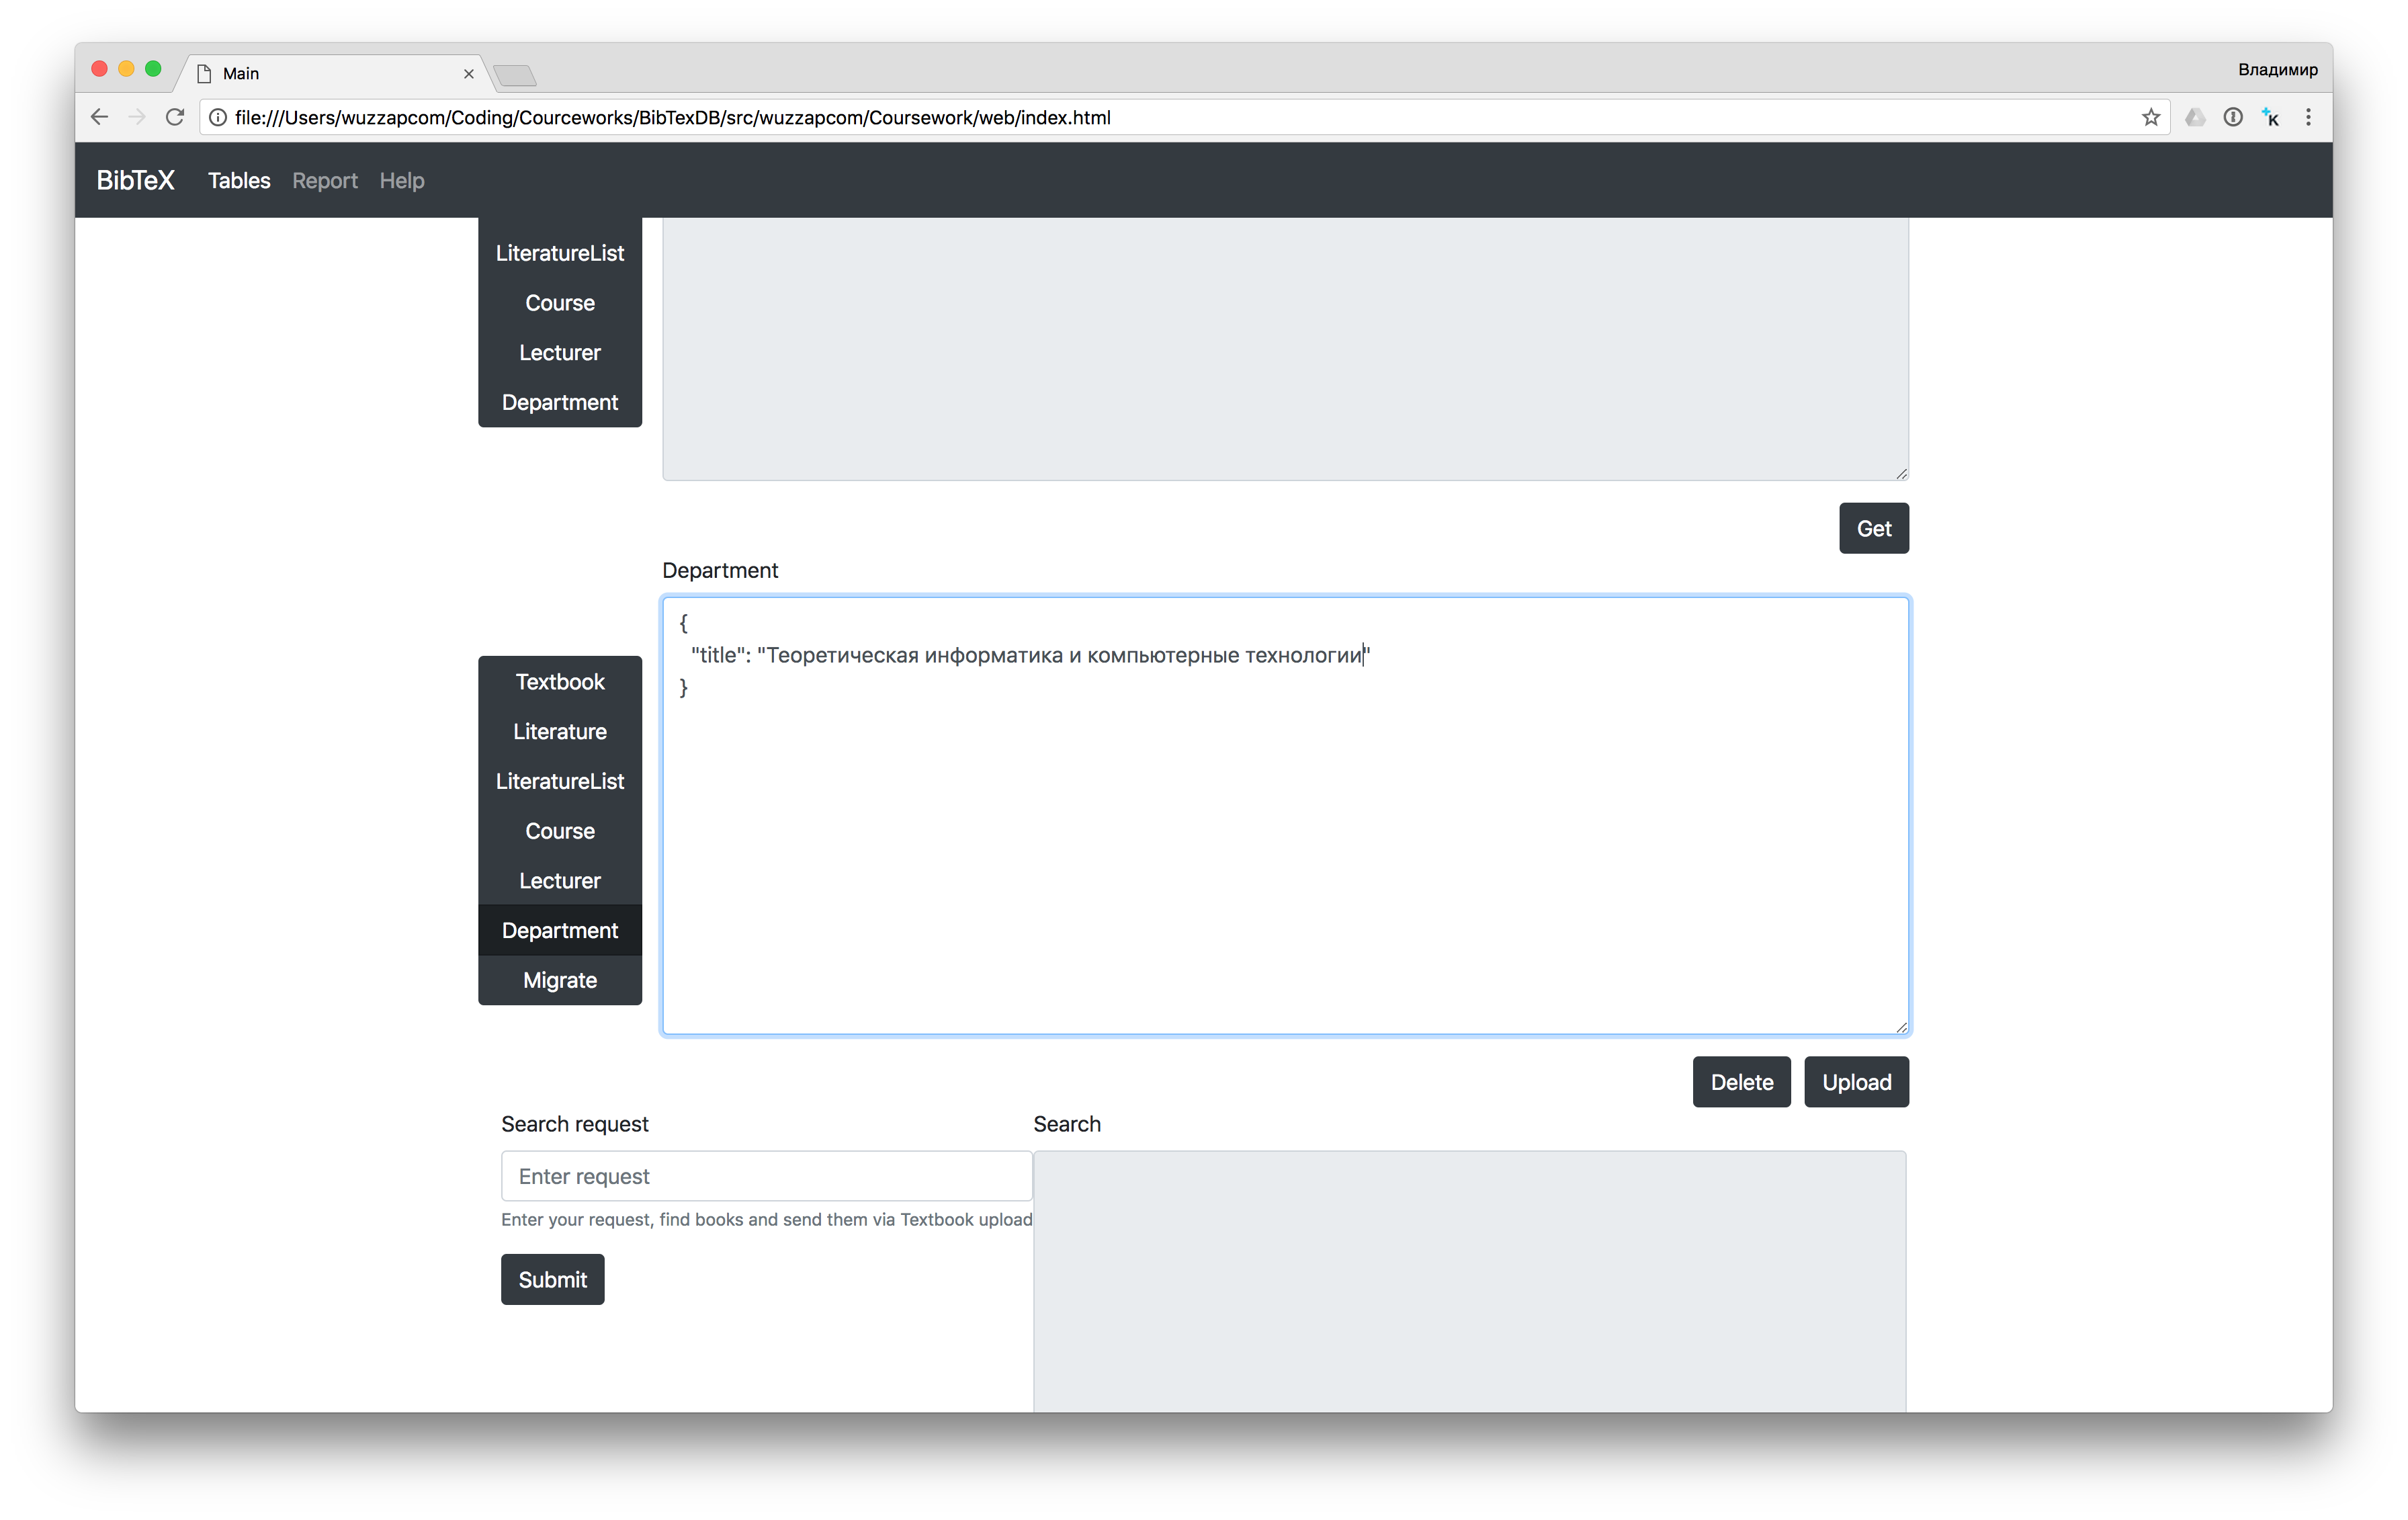
\includegraphics[width=1\linewidth]{web_add_department.png}}
	\caption{Добавление новой кафедры в веб-приложении}
	\label{web_add_department}
\end{figure}

Следующее действие -- добавление лектора к только что введенной кафедре. Последовательность действий
ничем не отличается от предыдущего шага и ее можно увидеть в листинге ~\ref{cli_add_lecturer} и рисунке
~\ref{web_add_lecturer}.

\begin{lstlisting}[language=bash, caption = {Добавление лектора}, captionpos=b, label={cli_add_lecturer}]
> cli lecturer prototype
Open lecturer.txt and fill prototype struct with correct data
> nano lecturer.txt 
> cli lecturer add
\end{lstlisting}

\begin{figure}[h!]
	\center{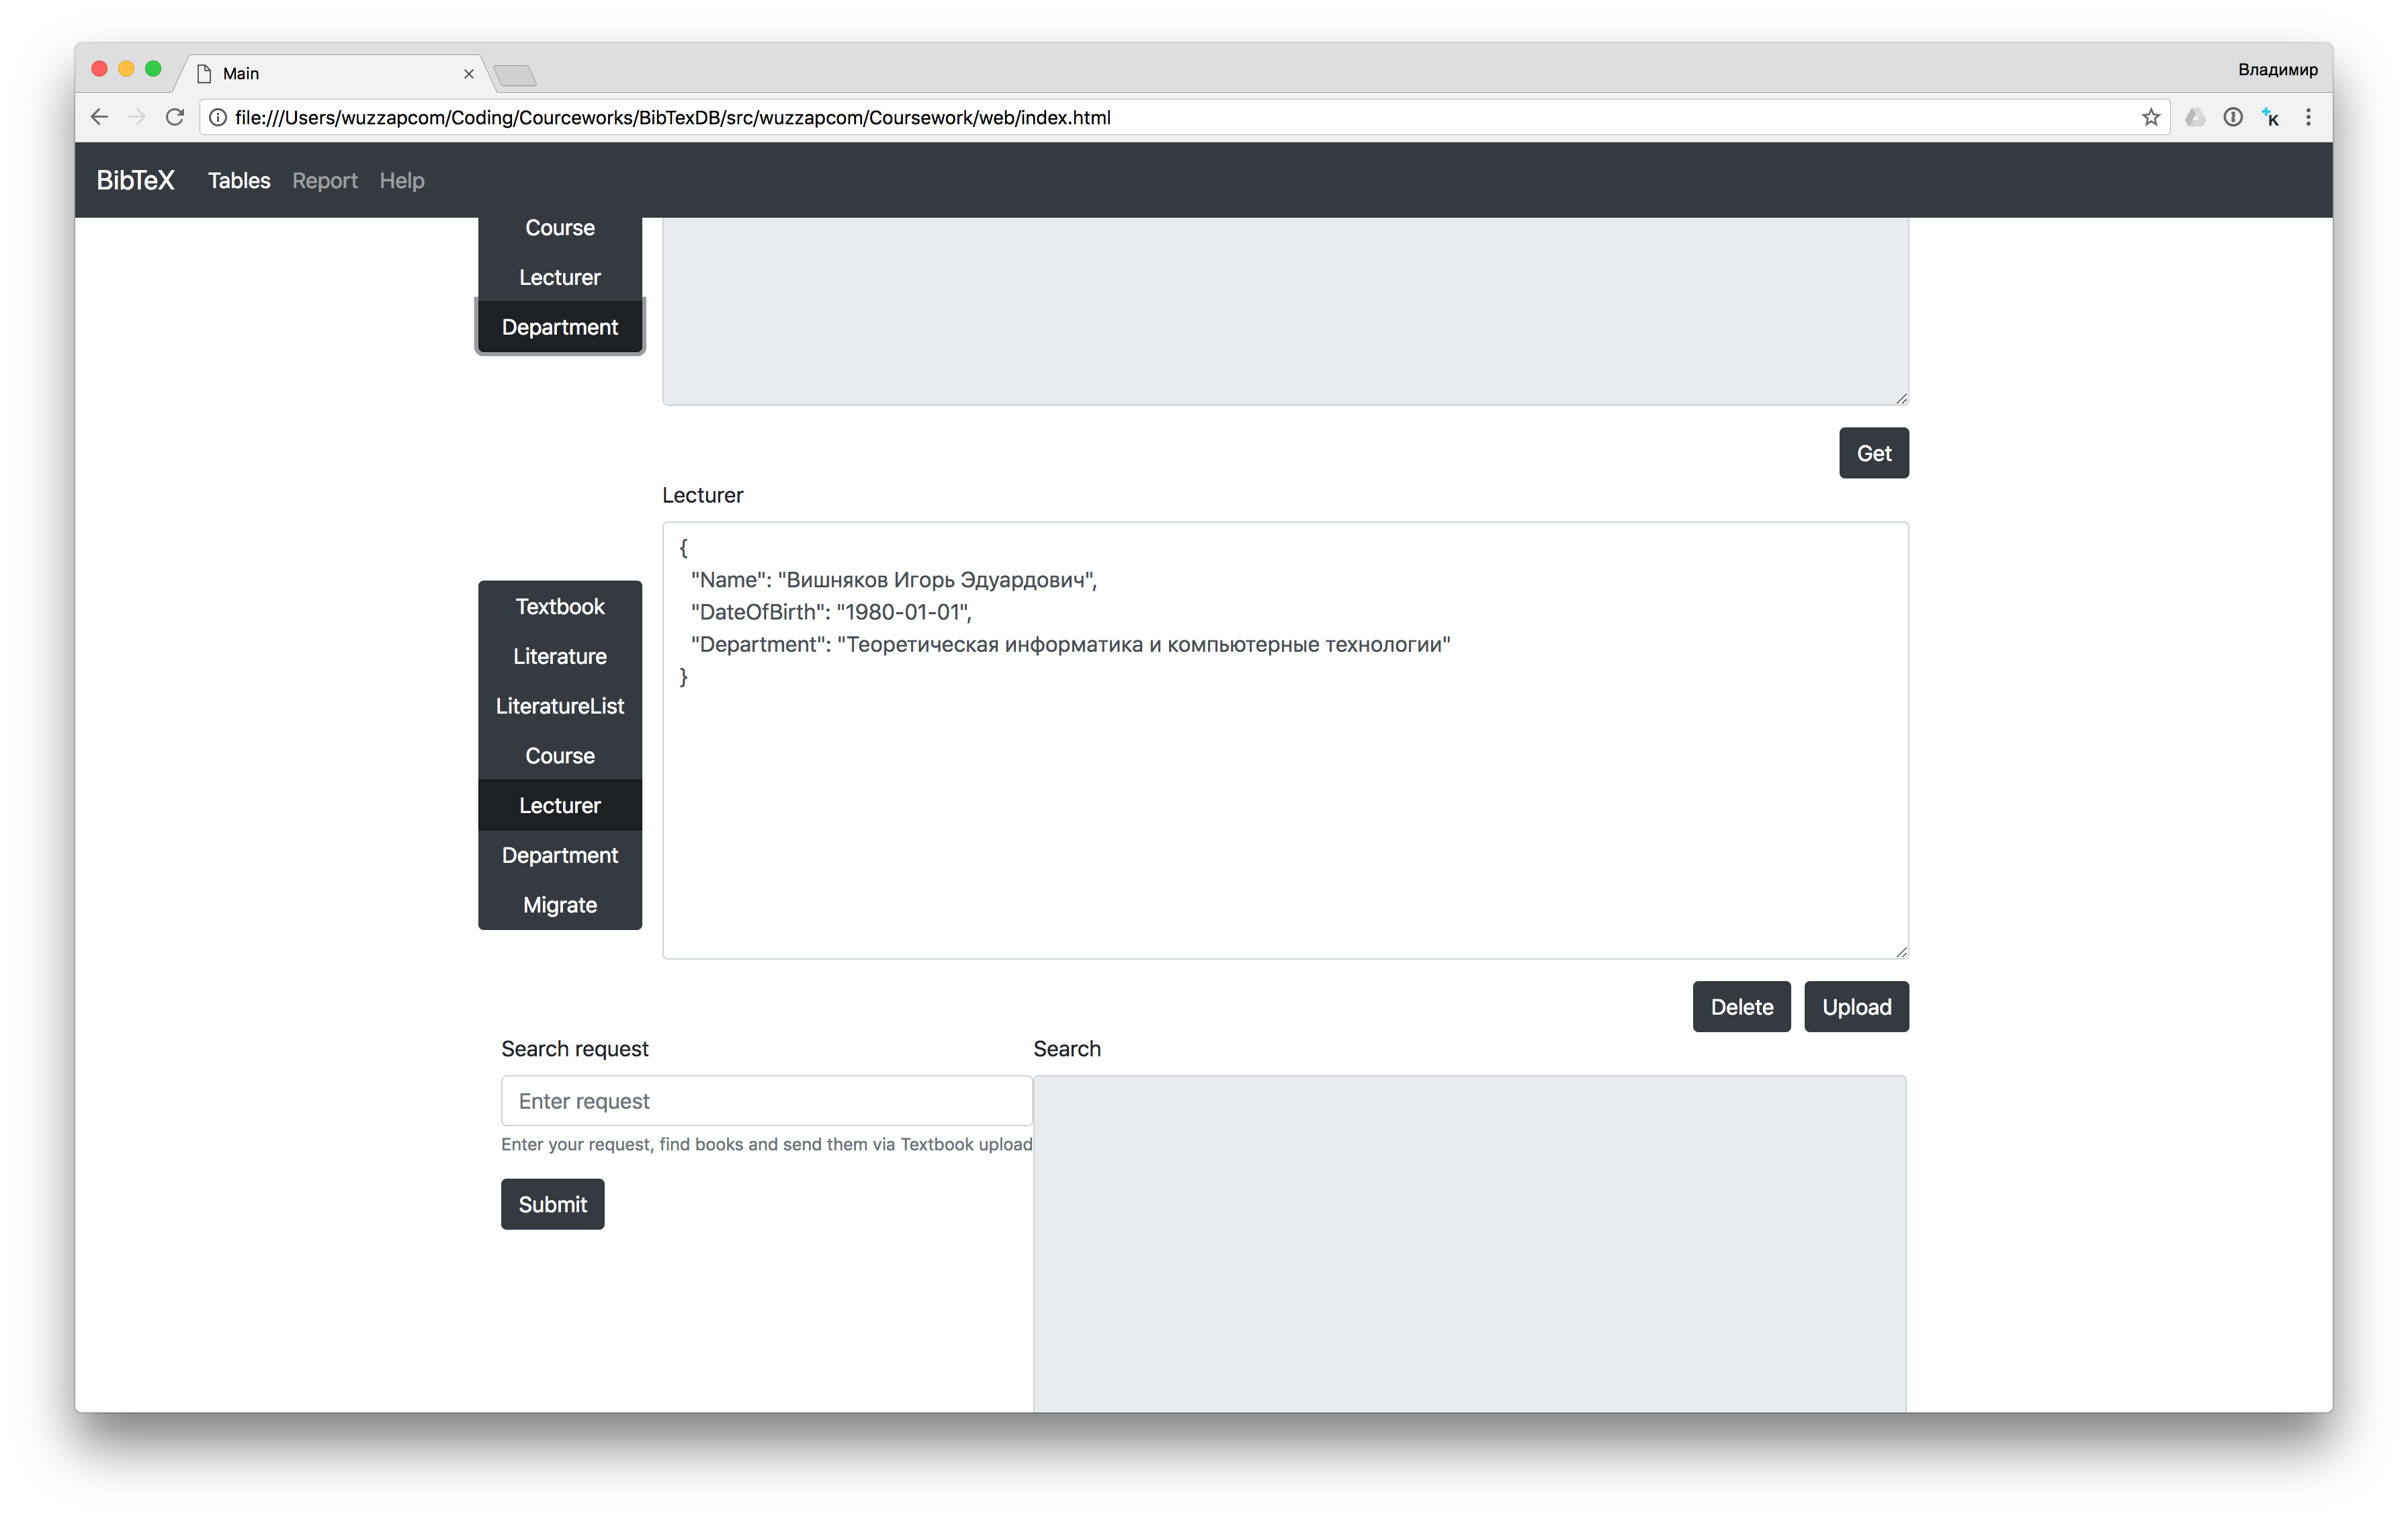
\includegraphics[width=1\linewidth]{web_add_lecturer.png}}
	\caption{Добавление нового лектора в веб-приложении}
	\label{web_add_lecturer}
\end{figure}

На шаге добавления курса становится видно преимущество веб-версии по сравнению с приложением командной строки.
Оно позволяет в двух разных окнах вводить информацию и делать запросы к базе данных. Иллюстрацию можно видеть
на рисунке ~\ref{web_add_course}. В этом примере можно держать перед глазами список добавленных лекторов чтобы,
например, не забыть дату рождения, и одновременно вводить данные об учебном курсе.

\begin{figure}[h!]
	\center{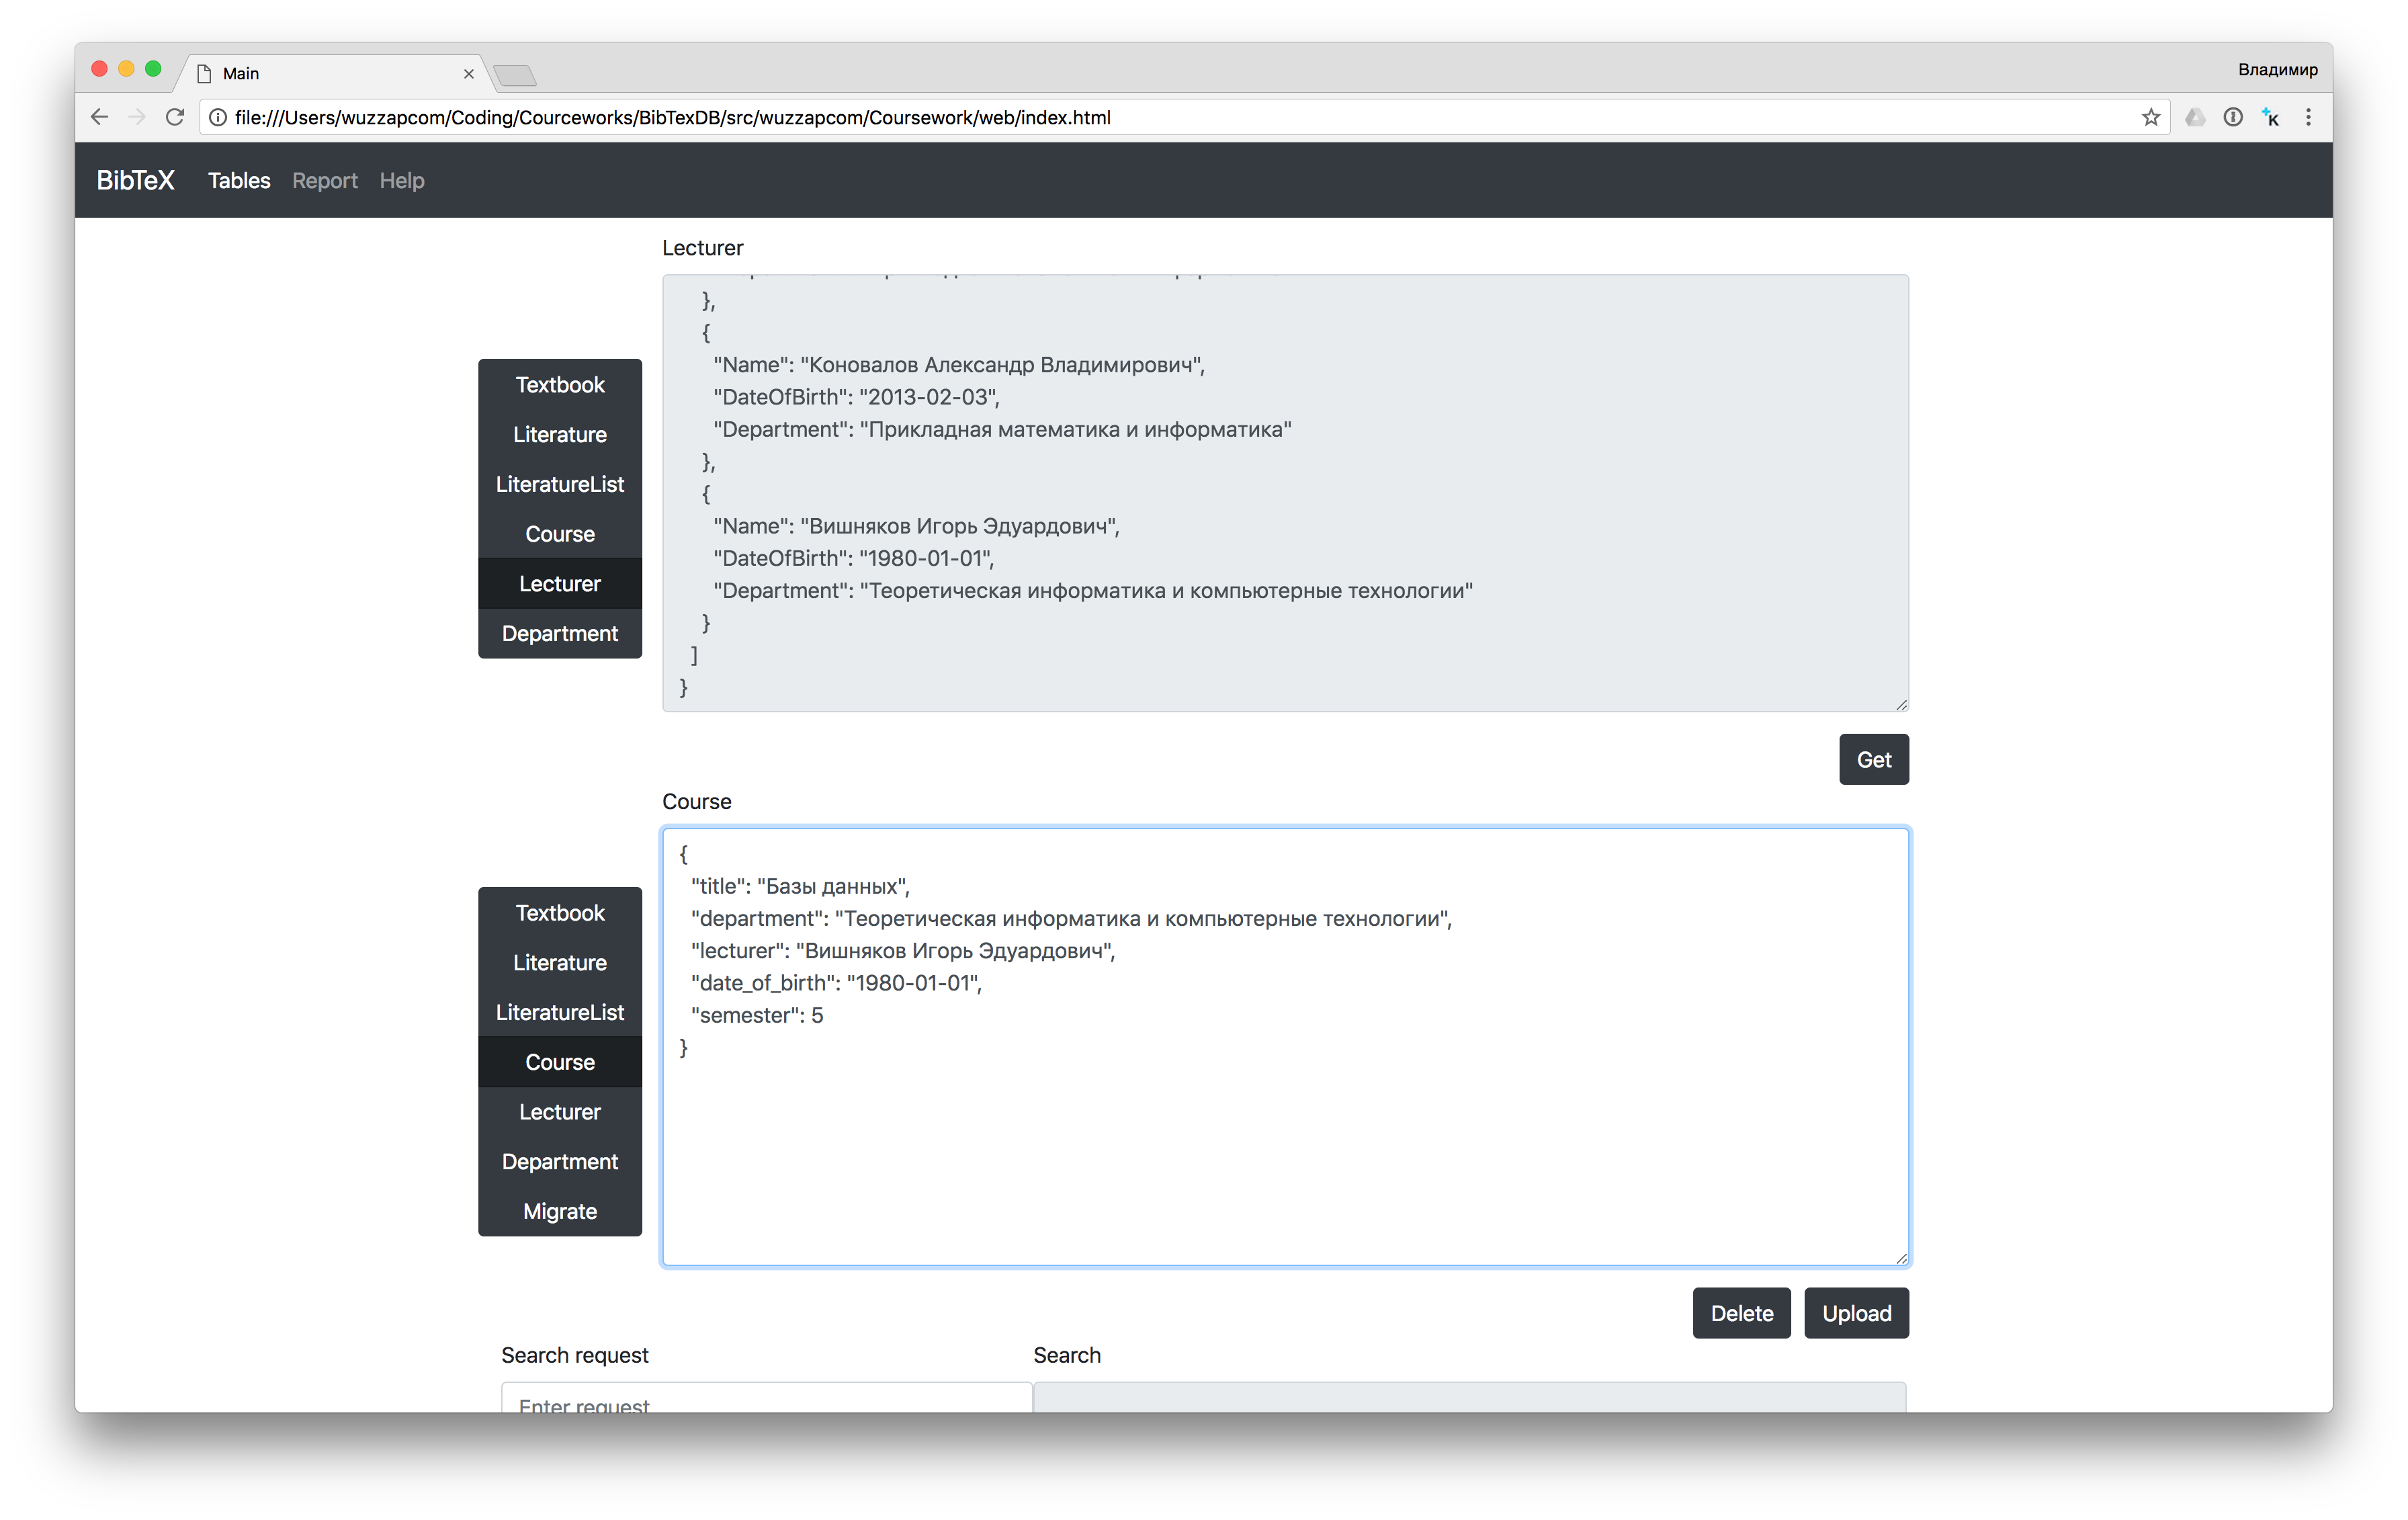
\includegraphics[width=1\linewidth]{web_add_course.png}}
	\caption{Добавление учебного курса в веб-приложении}
	\label{web_add_course}
\end{figure}

В то время как в приложении командной строки такой возможности нет. Как вариант, можно отдельно запросить список
лекторов командой \texttt{cli lector get}, чтобы открыть его в отдельном окне терминала или текстовом редакторе, но этот вариант 
явно проигрывает по удобству. Так что последовательность команд остается аналогичной и приведена в листинге ~\ref{cli_add_course}.

\begin{lstlisting}[language=bash, caption = {Добавление лектора}, captionpos=b, label={cli_add_course}]
> cli course prototype
Open course.txt and fill prototype struct with correct data
> nano course.txt 
> cli course add
\end{lstlisting}

Этап добавления нового учебного курса ничем не отличается от всех предыдущих, так что имеет смысл перейти к добавлению книг в приложение.
Как уже было сказано выше, для этого предусмотрен модуль, позволяющий использовать сервис Google Books для поиска информации о
книгах. Но возможно и добавление книг вручную, если нужного учебника не нашлось в базе сервиса. 
Для начала рассмотрим эту функцию в приложении командной строки из листинга ~\ref{cli_search}.

\begin{lstlisting}[language=bash, caption = {Поиск книг по запросу SQL в сервисе Google Books в приложении командной строки.}, captionpos=b, label={cli_search}]
> cli search --request="SQL"
Open searchResults.txt, view results, remove wrong 
items and fix incorrect data.
> nano searchResults.txt 
> cli book prototype
Open book.txt and fill prototype struct with correct data
> nano book.txt
> cli book add
\end{lstlisting}

Другими словами, необходимо сначала выполнить поиск, получить результат в файл, после чего скопировать нужную книгу в
\texttt{book.txt} и добавить ее командой \texttt{cli book add}.

Схожий принцип, но более удобный, используется и в веб-приложении, что можно увидеть на рисунке ~\ref{web_search}.

\begin{figure}[h!]
	\center{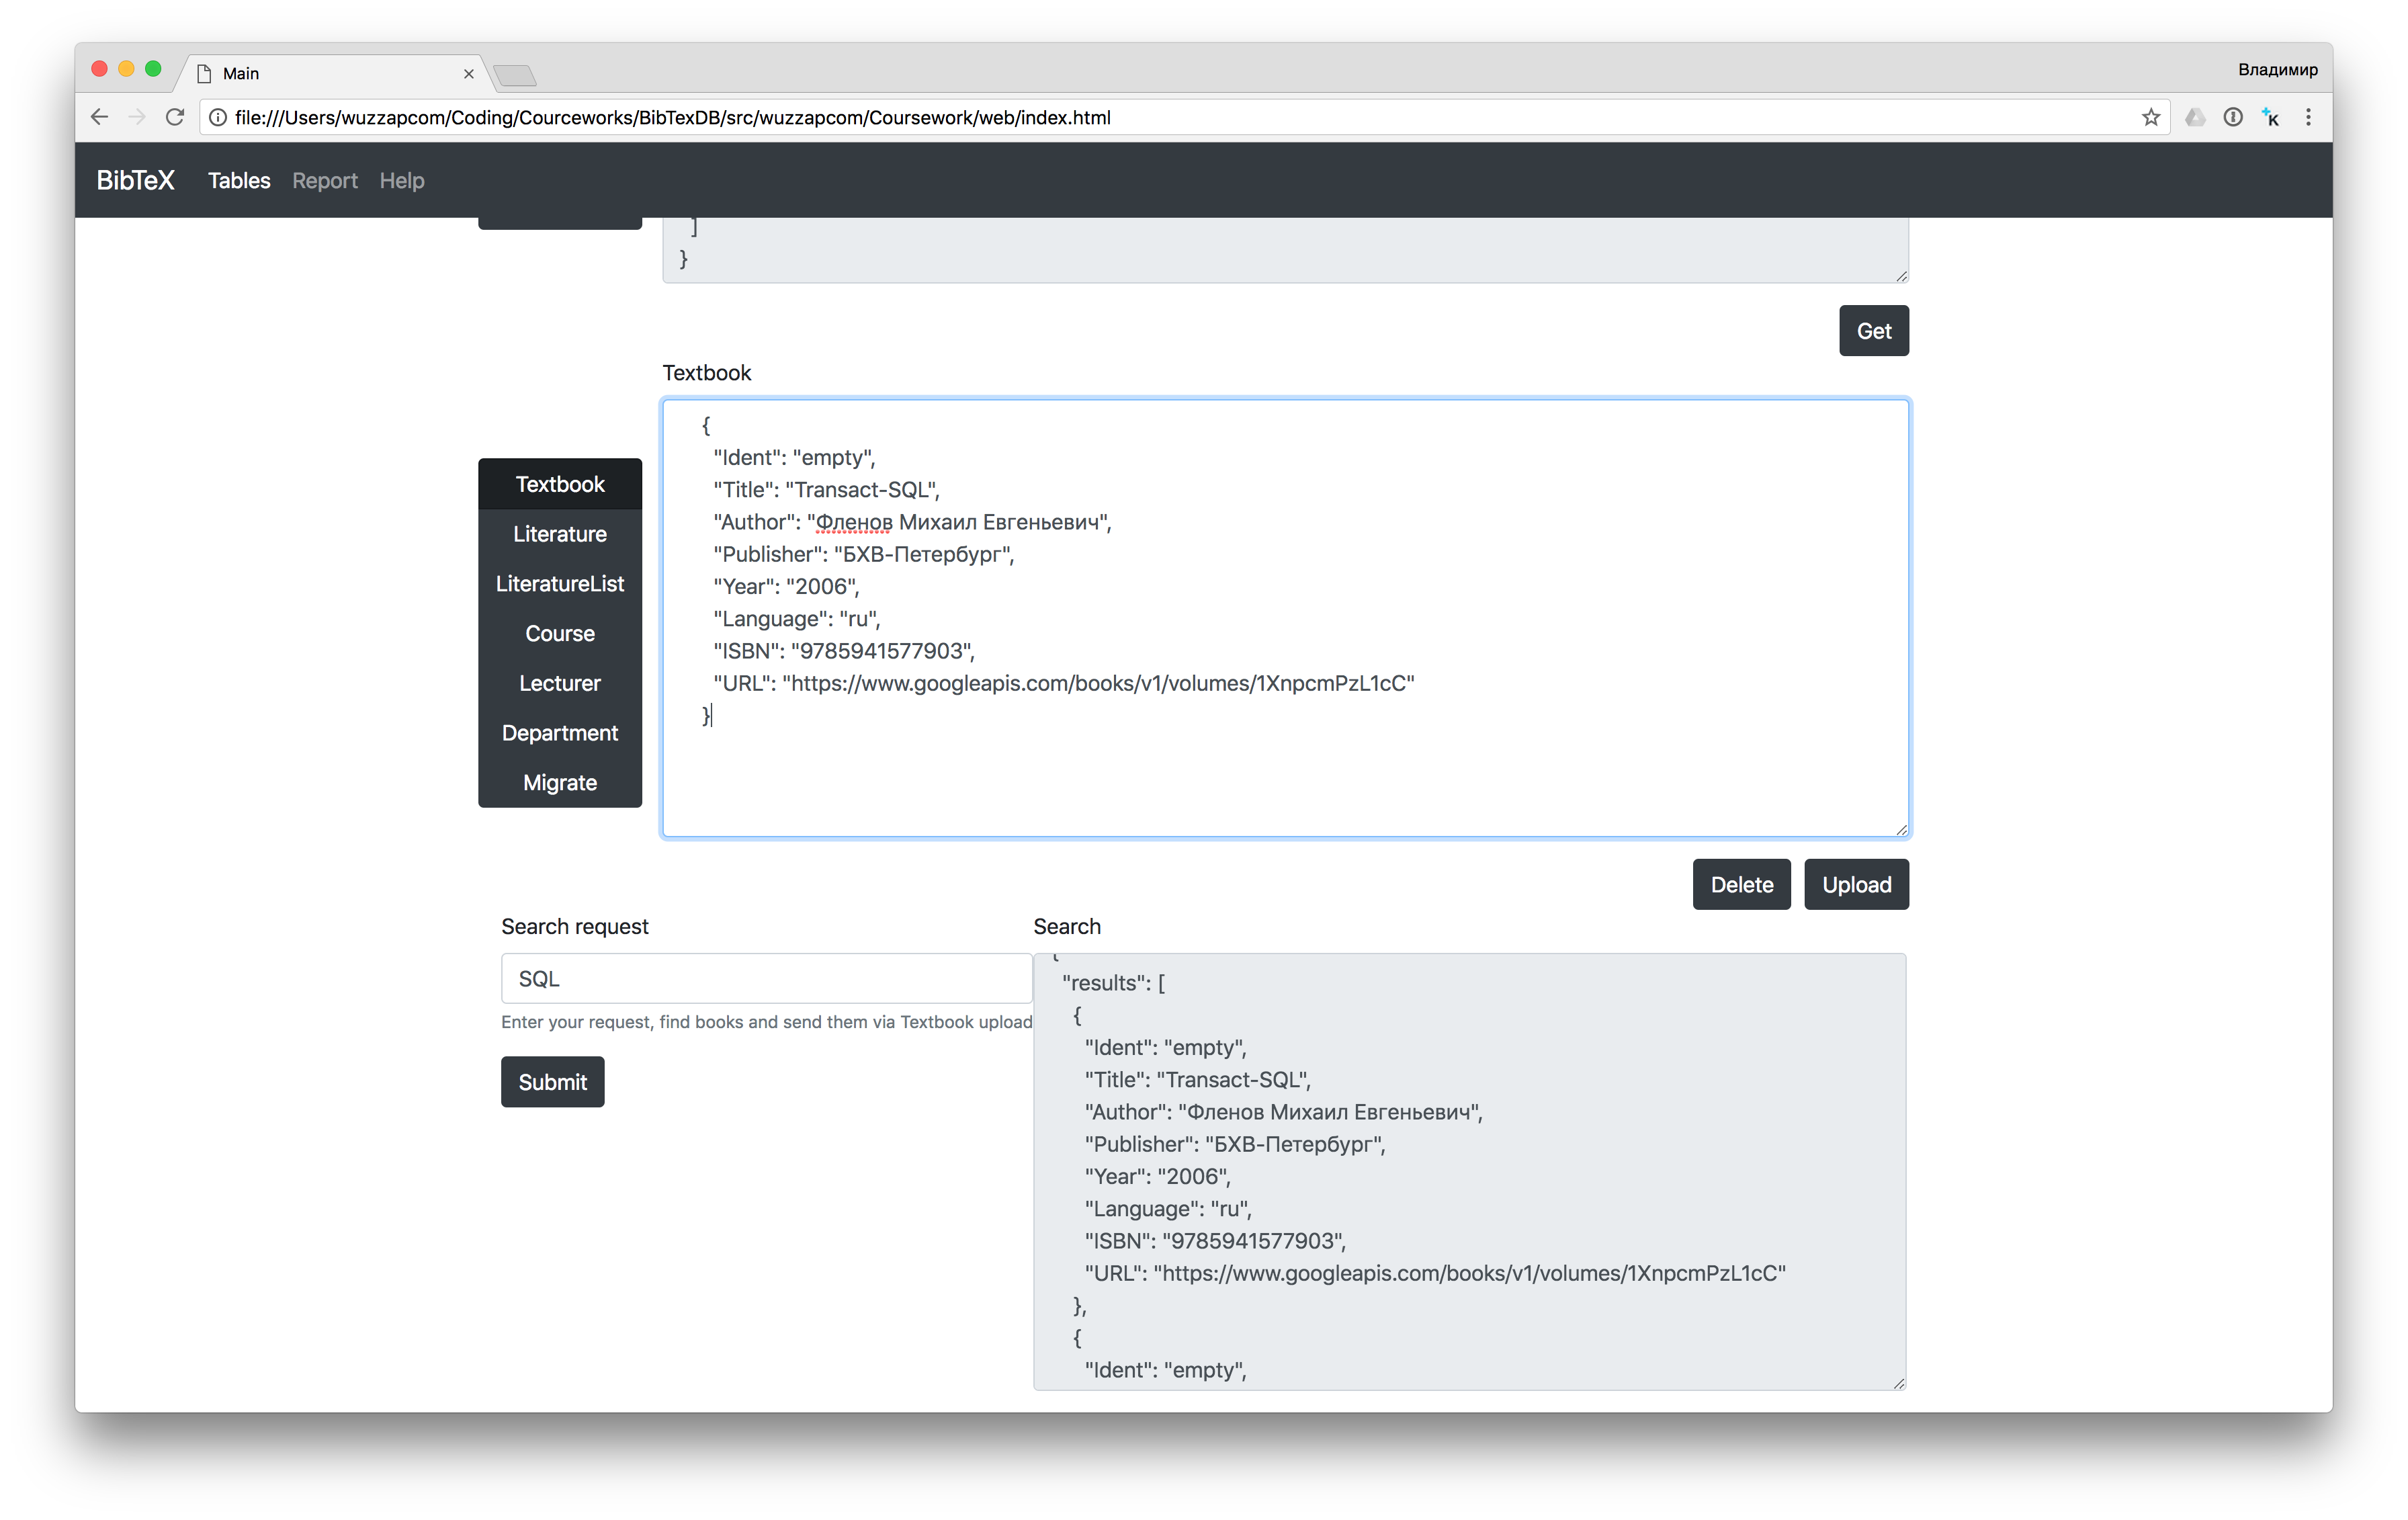
\includegraphics[width=1\linewidth]{web_search.png}}
	\caption{Поиск книг по запросу SQL в сервисе Google Books в веб-приложении.}
	\label{web_search}
\end{figure}

Добавление книги в список литературы также является набором тех же самых действий, так что имеет смысл перейти сразу к дополнительной функции:
миграции списков литературы. По своей сути, эта функция является абсолютно тем же заполнением нужной JSON-структуры, так что будет
удобно привести только вариант веб-приложения. Его можно видеть на рисунке ~\ref{web_migrate}

\begin{figure}[h!]
	\center{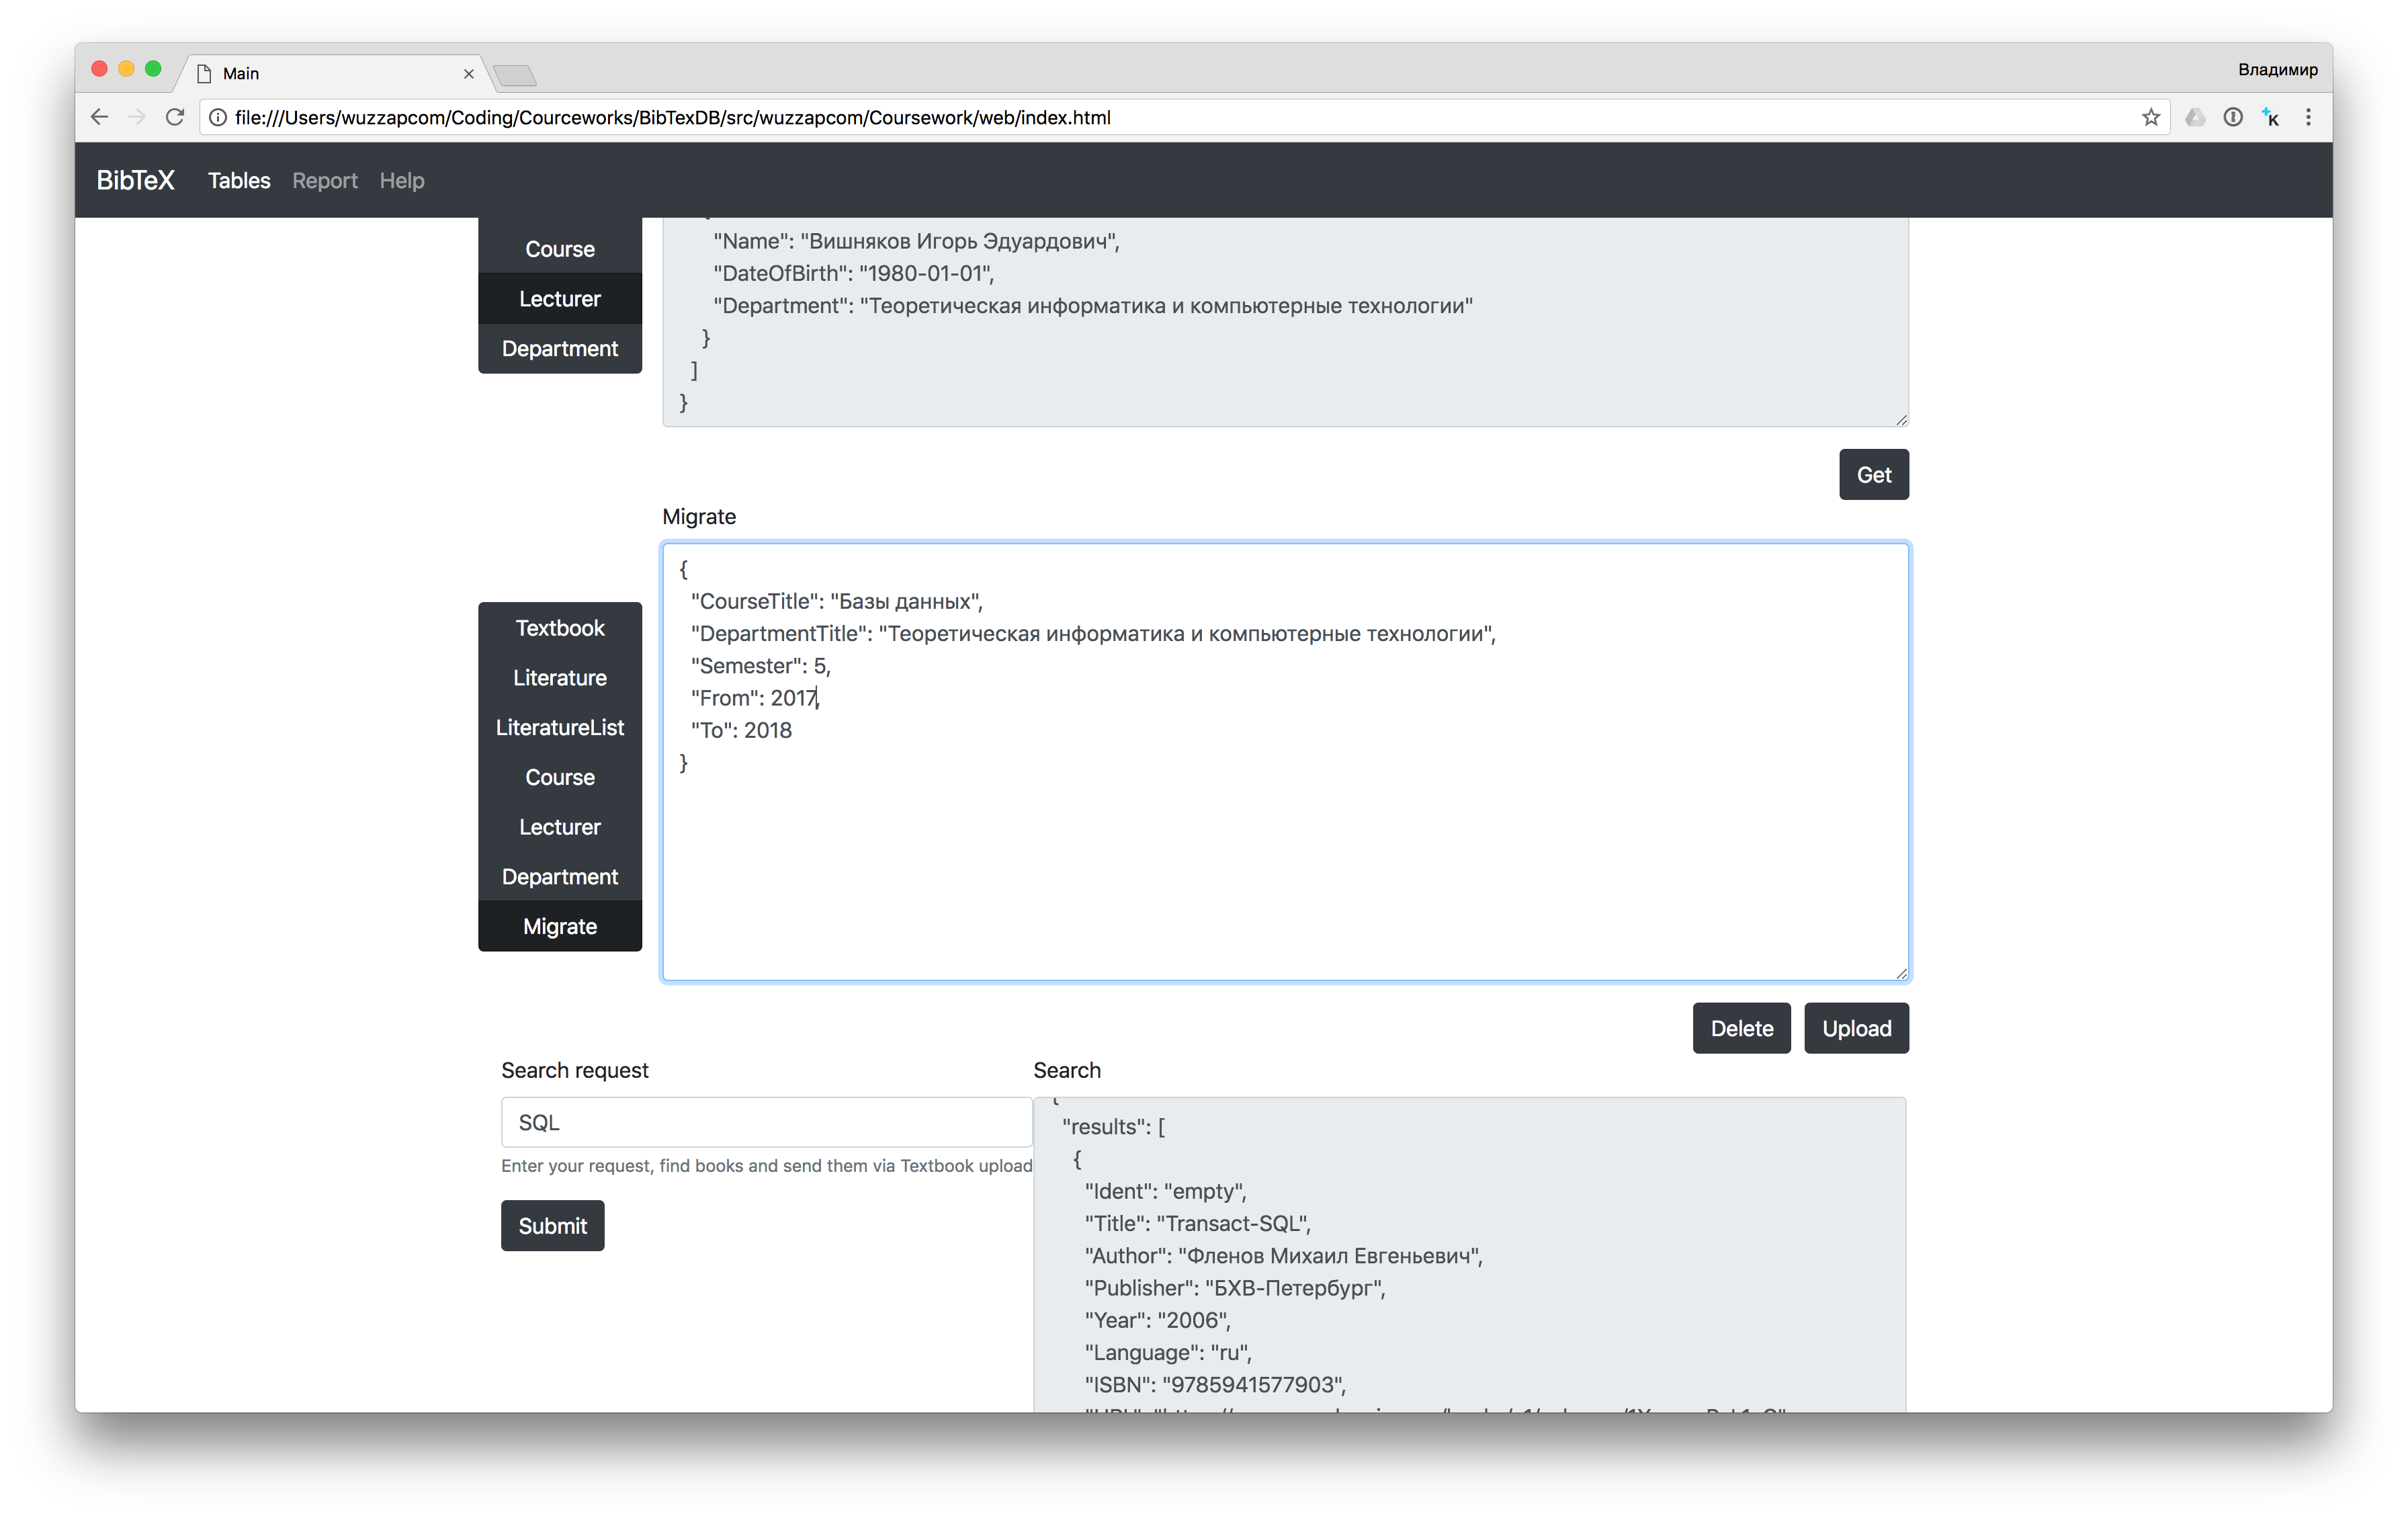
\includegraphics[width=1\linewidth]{web_migrate.png}}
	\caption{Демонстрация миграции списка литературы в веб-приложении.}
	\label{web_migrate}
\end{figure}

Важной деталью, которую необходимо отметить и зафиксировать, является то, что необходимо создать заранее тот список литературы, в который
будет производиться миграция.

Наконец стало возможным перейти к основному и самому важному пункту -- генерации самого отчета.

Для начала рассмотрим, как происходит генерация в приложении командной строки. Запрос необходимого отчета
происходит через отправку на сервер нужного списка литературы. Таким образом, запросить отчет можно последовательностью
команд из листинга ~\ref{cli_report}.

\begin{lstlisting}[language=bash, caption = {Запрос отчета в приложении командной строки.}, captionpos=b, label={cli_report}]
> cli literatureList prototype
Open literatureList.txt and fill prototype struct 
with correct data
> nano literatureList.txt
> cli report --outputFile="report.bib"
\end{lstlisting}

Как можно видеть, в команде \texttt{cli report} явным образом указан файл, в который будет записан результат. В случае
отсутствия этого флага отчет будет выведен в стандартный поток вывода, о чем сказано в справке данной команды.

Намного более удобно устроен весь процесс в веб-приложении. Специально для этого в нем сделано отдельное окно \texttt{Report}.
В нем отображаются все списки литературы, по нажатию на которые браузером сохраняется текстовый файл \texttt{report.bib}.
Рисунок ~\ref{web_report} демонстрирует данную функцию.

\begin{figure}[h!]
	\center{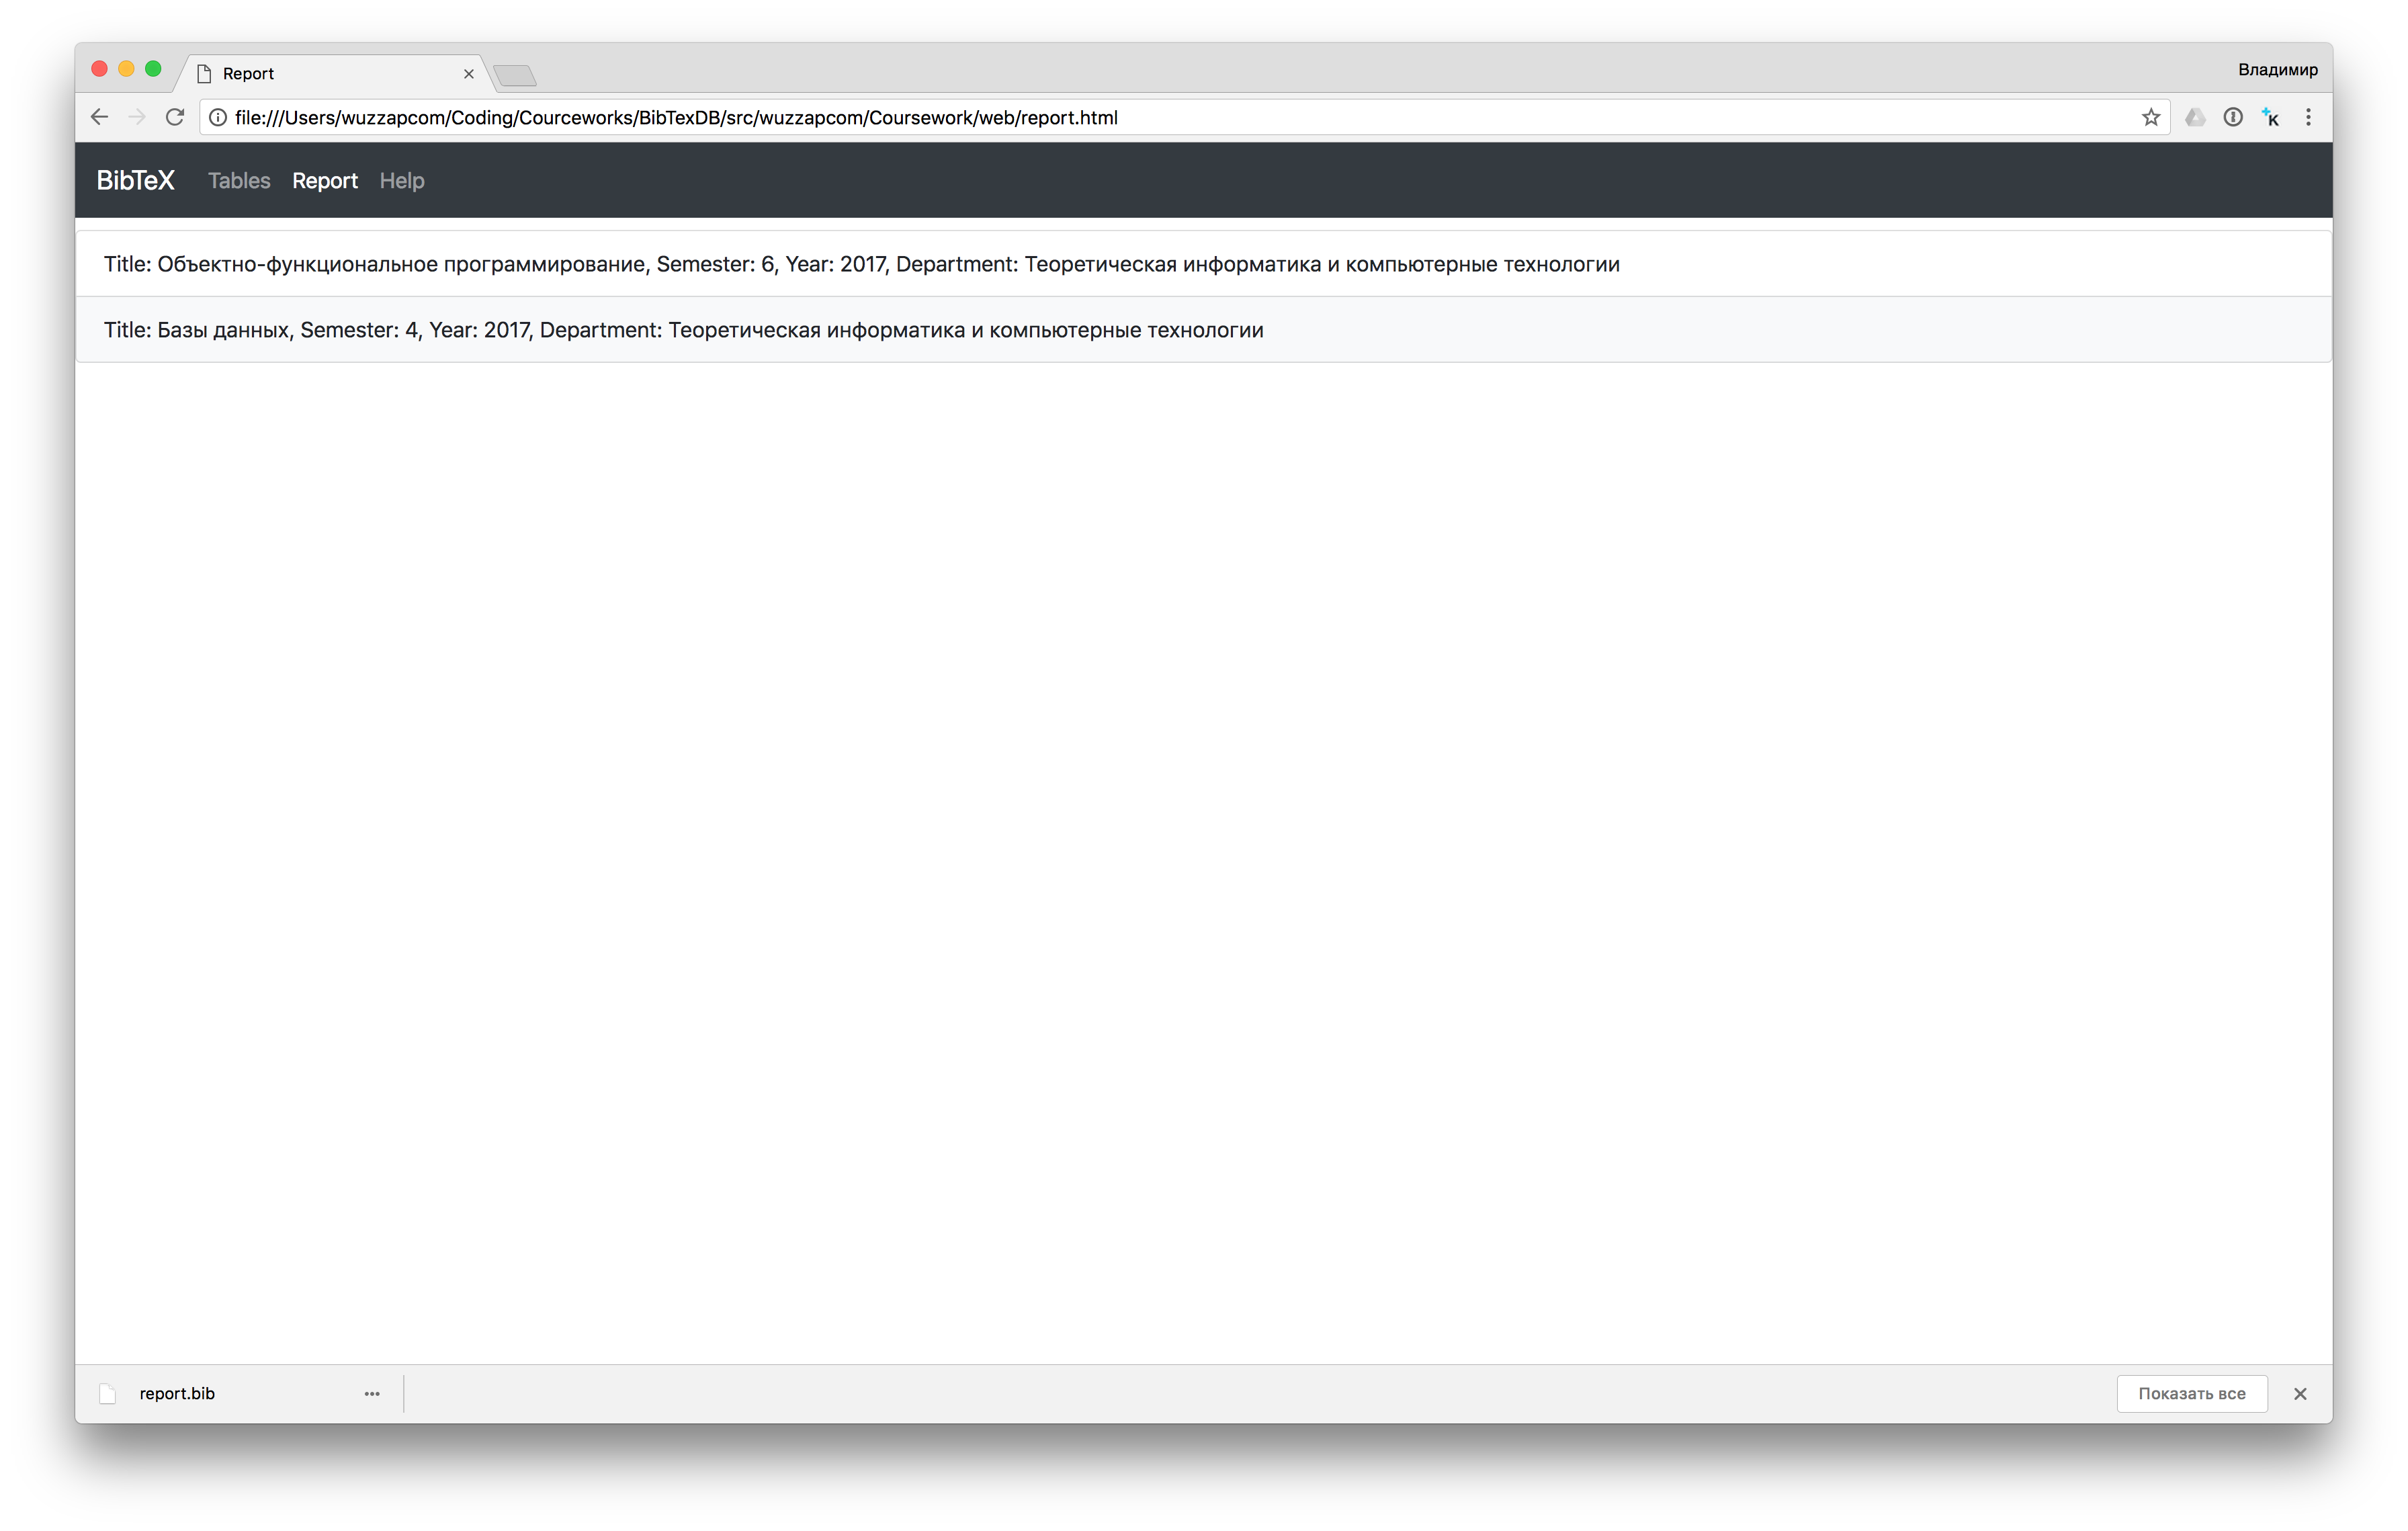
\includegraphics[width=1\linewidth]{web_report.png}}
	\caption{Демонстрация генерации отчета в веб-приложении.}
	\label{web_report}
\end{figure}

В качестве заключения хочется отметить, что работоспособность веб-приложения была проверена в браузерах Safari и Chrome на ноутбуке
под управлением операционной системы MacOS.

Таким образом, в данном разделе был рассмотрен полный цикл использования разработанного приложения, а также был продемонстрирован
принцип работы двух клиентских программ: веб-сайта и приложения командной строки. По результатам данного тестирования можно сказать, что
приложение командной строки выигрывает в автоматизируемости, но является неудобным при использовании человеком, в то время как 
веб-сайт, наоборот, предоставляет пользователю дополнительные функции для улучшения качества работы с разработанным приложением.

\clearpage
% -----------------

% Вывод
\section*{Заключение}
\addcontentsline{toc}{section}{Заключение}

В ходе данной курсовой работы был выполнен анализ и сравнение двух различных ветвей развития
систем управления базами данных: SQL и NoSQL, была произведена разработка серверного REST-приложения
с HTTP-интерфейсом.

Структура разработанного приложения выглядит следующим образом:

\begin{enumerate}
    \item База данных PostreSQL.
    \item Серверное приложение на языке Go с использованием драйвера для PostreSQL.
    \item Веб-сайт на языке TypeScript с использованием фреймворка Bootstrap.
    \item Приложение командной строки на языке Go с использованием фреймворка Cobra.
\end{enumerate}

Таким образом, было разработано приложение, выполняющее хранение и обработку информации о списках
литературы учебных курсов и была продемонстрирована его работоспособность на примере курса под
названием <<Базы данных>>.
\clearpage
% -----------------

% Список литературы
\renewcommand{\bibname}{Список использованной литературы}
\addcontentsline{toc}{section}{Список используемой литературы}
\bibliographystyle{unsrt}
\bibliography{literature}
% -----------------

\end{document}
